%TCIDATA{LaTeXparent=0,0,relatorio.tex}
                      
\chapter{Fundamenta��o Te�rica}\label{CapRevisaoBibliografica}

%[REVIS�O BIBLIOGR�FICA]
% Resumo opcional. Comentar se n�o usar.
%\resumodocapitulo{Resumo opcional.}

\section{Introdu��o}

Este cap�tulo destina-se a apresentar os componentes te�ricos que ir�o delinear o plano de fundo, a concep��o e a implementa��o do \textit{Smart Reservoir}. Inicialmente, s�o apresentados conceitos, aspectos operacionais e projetos de m�todos convencionais de recupera��o secund�ria de petr�leo, a maioria presente em \cite{engres} e \cite{engpetro}; a seguir, � dada uma introdu��o aos aspectos de simula��o num�rica de reservat�rios, t�pico que norteia a pr�pria implementa��o do algoritmo proposto nesta disserta��o. Ap�s a revis�o dos conceitos de engenharia de reservat�rio, procede-se aos conceitos matem�ticos b�sicos da teoria de otimiza��o e os principais algoritmos presentes na literatura; esses podem ser encontrados, por exemplo, em \cite{guller}, \cite{izmailov}, \cite{reklaitis} e \cite{yang}.
 
%TCIDATA{LaTeXparent=0,0,cap_RevisaoBibliografica.tex}

\section{M\'{e}todos Convencionais de Recupera\c{c}\~{a}o Secund\'{a}ria}

\subsection{Conceito e Contextualiza\c{c}\~{a}o da Recupera\c{c}\~{a}o Secund\'{a}ria}

De acordo com Rosa, nas acumula\c{c}\~{o}es de petr\'{o}leo h\'{a}, na \'{e}poca de sua descoberta, uma dada quantidade de energia, chamada de \textit{energia prim\'{a}ria}, cuja grandeza \'{e} determinada pelo volume e pela natureza dos fluidos existentes no meio, al\'{e}m dos n\'{i}veis de press\~{a}o e temperatura do reservat\'{o}rio; a quantidade de \'{o}leo retirada utilizando-se unicamente a energia do reservat\'{o}rio \'{e} denominada \textit{recupera\c{c}\~{a}o prim\'{a}ria} \cite{engres}. Haynes \textit{et al.} citam algumas formas de recupera\c{c}\~{a}o prim\'{a}ria, tais como: g\'{a}s em solu\c{c}\~{a}o, expans\~{a}o de g\'{a}s livre, influxo natural de \'{a}gua ou for\c{c}a gravitacional; os autores afirmam que a efici\^{e}ncia de recupera\c{c}\~{a}o prim\'{a}ria \'{e} menor nos processos envolvendo gases, maior em processos envolvendo \'{a}gua e gravita\c{c}\~{a}o, este \'{u}ltimo respons\'{a}vel pelos melhores resultados \cite{oil1976}.

Quando se d\'{a} o processo de produ\c{c}\~{a}o, parte da energia prim\'{a}ria \'{e} dissipada por causa da descompress\~{a}o dos fluidos do reservat\'{o}rio e das resist\^{e}ncias que os mesmos encontram ao fluir em dire\c{c}\~{a}o aos po\c{c}os produtores --- resist\^{e}ncias associadas \`{a}s for\c{c}as viscosas e capilares presentes no meio poroso \cite{engres}. Alotaibi afirma que essa energia \'{e} rapidamente depletada; a consequ\^{e}ncia dessa dissipa\c{c}\~{a}o de energia prim\'{a}ria resulta no decr\'{e}scimo de press\~{a}o do reservat\'{o}rio em sua vida produtiva e, consequentemente, na redu\c{c}\~{a}o da produtividade dos po\c{c}os \cite{alotaibi}. 

De forma a se minorar os efeitos danosos da dissipa\c{c}\~{a}o da energia prim\'{a}ria, existem duas linhas de a\c{c}\~{a}o a serem consideradas:

\begin{itemize}
\item Reduzir as resist\^{e}ncias viscosas e/ou capilares por meio de m\'{e}todos especiais, como por exemplo aquecendo a jazida;
\item Adicionar suplemento de energia secund\'{a}ria, artificialmente comunicada, atrav\'{e}s de inje\c{c}\~{a}o de fluidos em po\c{c}os selecionados.
\end{itemize}

Quando se suplementa o reservat\'{o}rio com energia transferida artificialmente, ou se empregam meios de incrementar a efici\^{e}ncia da energia prim\'{a}ria, a quantidade adicional de \'{o}leo produzida \'{e} chamada de \textit{recupera\c{c}\~{a}o secund\'{a}ria}. Por extens\~{a}o, todas as opera\c{c}\~{o}es que conduzem \`{a} obten\c{c}\~{a}o desse adicional de \'{o}leo tamb\'{e}m s\~{a}o denominadas recupera\c{c}\~{a}o secund\'{a}ria. Essas opera\c{c}\~{o}es, atualmente, s\~{a}o implantadas em sua grande maioria o t\~{a}o cedo quanto poss\'{i}vel na vida do reservat\'{o}rio.

\'{E} importante ressaltar que h\'{a} uma diferen\c{c}a entre recupera\c{c}\~{a}o secund\'{a}ria e m\'{e}todos de eleva\c{c}\~{a}o artificial e de estimula\c{c}\~{a}o de po\c{c}os; estes n\~{a}o afetam diretamente as energias expulsivas do reservat\'{o}rio, embora sua aplica\c{c}\~{a}o concorra para economiz\'{a}-las. As t\'{e}cnicas de eleva\c{c}\~{a}o artificial\footnote{Ver \cite{engpetro}.} e de estimula\c{c}\~{a}o de po\c{c}os est\~{a}o mais ligadas ao comportamento dos po\c{c}os produtores do que ao comportamento do reservat\'{o}rio como um todo. Contudo, a linha divis\'{o}ria entre tais m\'{e}todos e os m\'{e}todos de recupera\c{c}\~{a}o secund\'{a}ria n\~{a}o \'{e} muito n\'{i}tida --- certos m\'{e}todos de estimula\c{c}\~{a}o, como a inje\c{c}\~{a}o c\'{i}clica de vapor, s\~{a}o usualmente inclu\'{i}dos entre os m\'{e}todos de recupera\c{c}\~{a}o secund\'{a}ria \cite{engres}.

Ainda segundo Rosa, h\'{a} dois objetivos pr\'{a}ticos b\'{a}sicos dos m\'{e}todos de recupera\c{c}\~{a}o secund\'{a}ria:

\begin{itemize}
\item \textbf{Aumento da efici\^{e}ncia de recupera\c{c}\~{a}o} --- A efici\^{e}ncia de recupera\c{c}\~{a}o prim\'{a}ria \'{e} normalmente baixa; em alguns casos, dependendo das caracter\'{i}sticas do reservat\'{o}rio e dos fluidos, ela pode ser at\'{e} nula. Em alguns casos, a efici\^{e}ncia de recupera\c{c}\~{a}o secund\'{a}ria pode passar de 60\% em casos bem-sucedidos; contudo, o valor mais frequente dessa efici\^{e}ncia, nos m\'{e}todos convencionais, se situa entre 30 e 50\%.
\item \textbf{Acelera\c{c}\~{a}o da produ\c{c}\~{a}o} --- O emprego dos m\'{e}todos de recupera\c{c}\~{a}o secund\'{a}ria busca acelerar a produ\c{c}\~{a}o ou ao menos reduzir a taxa de seu decl\'{i}nio natural. A acelera\c{c}\~{a}o da produ\c{c}\~{a}o resulta em antecipa\c{c}\~{a}o do fluxo de caixa; portanto, h\'{a} o aumento de seu valor presente e uma consequente melhoria da economicidade da explora\c{c}\~{a}o do campo ou reservat\'{o}rio.
\end{itemize}

Al\'{e}m dos objetivos b\'{a}sicos de emprego da recupera\c{c}\~{a}o secund\'{a}ria, ha v\'{a}rios outros incentivos ao uso desses m\'{e}todos, tais como: pre\c{c}o do petr\'{o}leo; custos de explora\c{c}\~{a}o, desenvolvimento e produ\c{c}\~{a}o; e avan\c{c}os tecnol\'{o}gicos na \'{a}rea. Por\'{e}m, destaca-se que apenas o uso dessas t\'{e}cnicas n\~{a}o \'{e} o suficiente para mitigar todos os males da produ\c{c}\~{a}o de petr\'{o}leo e do esgotamento das reservas; outras medidas podem e devem ser tomadas, simultaneamente, para aumentar a efici\^{e}ncia e a rentabilidade da produ\c{c}\~{a}o, tais como\footnote{Ver \cite{engres}}:
%TODO encontrar as paginas do Rosa para essa parte
\begin{itemize}
\item \textbf{Explora\c{c}\~{a}o de reservas n\~{a}o convencionais} --- Xistos e folhelhos betuminosos, por exemplo, acumulam grandes quantidades de \'{o}leo. V\'{a}rias dessas reservas j\'{a} foram encontradas em regi\~{o}es como Athabasca, no Canad\'{a}, cintur\~{a}o do Orinoco, na Venezuela, e o Colorado, nos Estados Unidos. O custo de produ\c{c}\~{a}o nessas reservas \'{e} consider\'{a}vel, mas j\'{a} se projetam meios tecnol\'{o}gicos para reduzir o mesmo. Entre outras reservas n\~{a}o convencionais de hidrocarbonetos, h\'{a} a presen\c{c}a de g\'{a}s natural em solu\c{c}\~{a}o existente na \'{a}gua de aqu\'{i}feros; embora a raz\~{a}o de solubilidade do g\'{a}s natural na \'{a}gua normalmente seja pequena, o imenso volume dos aqu\'{i}feros perimitiria uma produ\c{c}\~{a}o de grandes volumes desse g\'{a}s. Uma outra reserva n\~{a}o convecional poder\'{a} ser o g\'{a}s natural proveniente de hidratos localizados no fundo de oceanos e em regi\~{o}es congeladas da Terra.
\item \textbf{Estimula\c{c}\~{a}o de Po\c{c}os} De acordo com Thomas, a estimula\c{c}\~{a}o de po\c{c}os \'{e} um conjunto de atividades realizadas com o objetivo de aumentar o \'{i}ndice de produtividade ou injetividade do po\c{c}o \cite[p.~166]{engpetro}. Os principais m\'{e}todos de estimula\c{c}\~{a}o s\~{a}o: fraturamento hidr\'{a}ulico, em que se cria, atrav\'{e}s de uma ruptura na rocha-reservat\'{o}rio causada por um elevado gradiente de press\~{a}o, um caminho preferencial de alta condutividade, facilitando um fluxo de fluidos do reservat\'{o}rio ao po\c{c}o (ou vice-versa); e acidifica\c{c}\~{a}o, onde se injeta um \'{a}cido com press\~{a}o inferior \`{a} press\~{a}o de fraturamento da forma\c{c}\~{a}o, visando remover danos da mesma. Tais m\'{e}todos contribuem para a acelera\c{c}\~{a}o da produ\c{c}\~{a}o e at\'{e}, em alguns casos, o aumento da efici\^{e}ncia de recupera\c{c}\~{a}o. A aplica\c{c}\~{a}o de m\'{e}todos de estimula\c{c}\~{a}o pode, inclusive, ser feita em campos submetidos a opera\c{c}\~{o}es de recupera\c{c}\~{a}o secund\'{a}ria.
\item \textbf{Uso de po\c{c}os especiais} --- Nas \'{u}ltimas d\'{e}cadas houve um incremento consider\'{a}vel no uso dos chamados \textit{po\c{c}os especiais}, que possuem como caracter\'{i}stica marcante a n\~{a}o-verticalidade, Segundo Thomas, esses po\c{c}os s\~{a}o perfurados com v\'{a}rias finalidades, como: controlar um po\c{c}o em \textit{blowout} por meio de po\c{c}os de al\'{i}vio; atingir forma\c{c}\~{o}es produtoras abaixo de locais inacess\'{i}veis, como rios, lagos, cidades, entre outros; desviar a trajet\'{o}ria do po\c{c}o de acidentes geol\'{o}gicos, como domos salinos e falhas; perfurar v\'{a}rios po\c{c}os de um mesmo ponto, como \'{e} o caso da produ\c{c}\~{a}o em plataformas mar\'{i}timas; e desviar po\c{c}os que tiveram seu trecho final perdido por problemas operacionais \cite[p. 106]{engpetro}. O uso desses po\c{c}os inclinados, horizontais, multilaterais, etc., pode aumentar a velocidade de drenagem do reservat\'{o}rio, ou seja, antecipar a produ\c{c}\~{a}o, bem como aumentar a efici\^{e}ncia de recupera\c{c}\~{a}o atrav\'{e}s do aumento da efici\^{e}ncia de varrido, por exemplo.
\item \textbf{Extra\c{c}\~{a}o de l\'{i}quidos de g\'{a}s natural} --- A produ\c{c}\~{a}o de hidrocarbonetos l\'{i}quidos pode ser aumentada pela instala\c{c}\~{a}o de plantas de gasolina natural e de unidades port\'{a}teis de extra\c{c}\~{a}o de l\'{i}quidos de g\'{a}s natural.
\item \textbf{Reestudo de \'{a}reas julgadas improdutivas ou antiecon\^{o}micas} --- Mesmo que as reservas mundiais de petr\'{o}leo sejam limitadas, elas est\~{a}o longe de terem sido totalmente exploradas; de fato, apenas uma pequena porcentagem da superf\'{i}cie do planeta foi inteiramente explorada. Seja na terra ou no fundo do mar, h\'{a} ainda perspectivas not\'{a}veis fora das \'{a}reas hoje em produ\c{c}\~{a}o; al\'{e}m disso, as estimativas do volume de \'{o}leo que ainda poder\'{a} ser descoberto s\~{a}o ainda vagas. \'{E} com essa perspectiva que a ind\'{u}stria pode medir as oportunidades que tem \`{a} frente no caso de esgotamento das \'{a}reas hoje em produ\c{c}\~{a}o. Portanto, de um modo geral, deve-se pensar sempre na ado\c{c}\~{a}o das seguintes medidas, sem danos ao andamento das opera\c{c}\~{o}es de recupera\c{c}\~{a}o secund\'{a}ria: estudar novas \'{a}reas; estudar forma\c{c}\~{o}es mais profundas (o pr\'{e}-sal \'{e} um exemplo); reestudar \'{a}reas consideradas esgotadas ou de produ\c{c}\~{a}o antiecon\^{o}mica; e investir mais dinheiro, tempo e pessoal em treinamento e pesquisa, visando melhorar os m\'{e}todos de explora\c{c}\~{a}o e produ\c{c}\~{a}o existentes.
\end{itemize}

\subsection{Classifica\c{c}\~{a}o dos M\'{e}todos de Recupera\c{c}\~{a}o Secund\'{a}ria}
Segundo Rosa, os m\'{e}todos de recupera\c{c}\~{a}o de \'{o}leo visando suplementar a energia do reservat\'{o}rio, logo ap\'{o}s a fase de recupera\c{c}\~{a}o prim\'{a}ria, eram denominados, originalmente, m\'{e}todos de recupera\c{c}\~{a}o secund\'{a}ria, enquanto que m\'{e}todos empregados posteriormente passaram a ser chamados de \textit{recupera\c{c}\~{a}o terci\'{a}ria}; Alotaibi afirma que os m\'{e}todos de recupera\c{c}\~{a}o terci\'{a}ria s\~{a}o utilizados para se recuperar \'{o}leo residual logo ap\'{o}s o emprego de t\'{e}cnicas como a inje\c{c}\~{a}o de \'{a}gua \cite{alotaibi}. Adeniyi \textit{et al.} afirmam que a recupera\c{c}\~{a}o terci\'{a}ria reduz a viscosidade do \'{o}leo para incrementar sua produ\c{c}\~{a}o; os autores destacam que tais m\'{e}todos tamb\'{e}m podem ser utilizados caso haja componentes de \'{o}leo cru pesado \cite{adeniyi2008}. 

Os m\'{e}todos tamb\'{e}m podiam ser classificados de acordo com a sua cronologia de aplica\c{c}\~{a}o em determinado campo ou reservat\'{o}rio. Posteriormente, todos os m\'{e}todos de recupera\c{c}\~{a}o aplicados com o objetivo de aumentar a efici\^{e}ncia de recupera\c{c}\~{a}o e/ou acelerar a produ\c{c}\~{a}o em rela\c{c}\~{a}o \`{a} produ\c{c}\~{a}o prim\'{a}ria passaram a ser denominados de recupera\c{c}\~{a}o secund\'{a}ria.

Nas \'{u}ltimas d\'{e}cadas, a classifica\c{c}\~{a}o dos m\'{e}todos de recupera\c{c}\~{a}o secund\'{a}ria se deu em \textit{m\'{e}todos convencionais} (os antigos m\'{e}todos de recupera\c{c}\~{a}o secund\'{a}ria) e \textit{m\'{e}todos especiais} (os antigos m\'{e}todos de recupera\c{c}\~{a}o terci\'{a}ria), os \'{u}ltimos tamb\'{e}m conhecidos, na literatura inglesa, como m\'{e}todos de \textit{EOR} (\textit{Enhanced Oil Recovery}) --- esse termo, nos \'{u}ltimos anos, tem sido substitu\'{i}do pelo termo \textit{IOR} (\textit{Improved Oil Recovery}), cuja diferen\c{c}a, em rela\c{c}\~{a}o ao \textit{EOR}, reside no fato de que os m\'{e}todos de \textit{IOR} englobam, al\'{e}m dos m\'{e}todos de \textit{EOR}, quaisquer m\'{e}todos ou t\'{e}cnicas n\~{a}o-convencionais ou modernas que possuam o objetivo de aumentar a produ\c{c}\~{a}o e/ou acelerar a produ\c{c}\~{a}o em rela\c{c}\~{a}o \`{a} produ\c{c}\~{a}o prim\'{a}ria e/ou secund\'{a}ria \cite[p. 564]{engres}. 

O estudo das t\'{e}cnicas de EOR concentrou esfor\c{c}os de v\'{a}rios pesquisadores, desde a d\'{e}cada de 1970, em que tais m\'{e}todos se tornaram populares \cite{coats1982}; Udy \textit{et al.} destacam o uso dessas t\'{e}cnicas acopladas a m\'{e}todos de otimiza\c{c}\~{a}o para se tentar maximizar a produ\c{c}\~{a}o de petr\'{o}leo \cite{udyEOR}; Ling \textit{et al.} analisam a implementa\c{c}\~{a}o e o efeito de v\'{a}rias t\'{e}cnicas de EOR na Forma\c{c}\~{a}o de Bakken, situada na Depress\~{a}o de Williston, EUA, de maneira a se utilizar o melhor m\'{e}todo na quest\~{a}o da recupera\c{c}\~{a}o de \'{o}leo \cite{ling2014}; Alvarado e Manrique apresentam a evolu\c{c}\~{a}o de alguns m\'{e}todos de EOR ao longo dos anos, e afirmam que as t\'{e}cnicas de IOR, al\'{e}m de emcompassarem as de EOR, incluem novas tecnologias de perfura\c{c}\~{a}o e de po\c{c}os, administra\c{c}\~{a}o e controle inteligente de reservat\'{o}rios, t\'{e}cnicas de monitoramento avan\c{c}ado de reservat\'{o}rios, al\'{e}m de aplica\c{c}\~{o}es de diferentes melhorias de processos de recupera\c{c}\~{a}o prim\'{a}ria e secund\'{a}ria \cite{alvarado2010}.

Em termos da classifica\c{c}\~{a}o mais atual, s\~{a}o m\'{e}todos convencionais de recupera\c{c}\~{a}o secund\'{a}ria os m\'{e}todos de inje\c{c}\~{a}o de \'{a}gua e inje\c{c}\~{a}o imisc\'{i}vel de g\'{a}s. J\'{a} os m\'{e}todos especiais incluem, entre outros, a inje\c{c}\~{a}o misc\'{i}vel de g\'{a}s, a inje\c{c}\~{a}o de vapor, a inje\c{c}\~{a}o de pol\'{i}meros e a combust\~{a}o \textit{in situ}\footnote{Tais m\'{e}todos s\~{a}o citados em \cite{oil1976}. Uma abordagem sobre os m\'{e}todos especiais pode ser encontrada em \cite[pp. 677-726]{engres}}. A Figura \ref{fig:recreview} destaca os m\'{e}todos mais comuns de recupera\c{c}\~{a}o.

\begin{figure}[!ht]
	\centering
	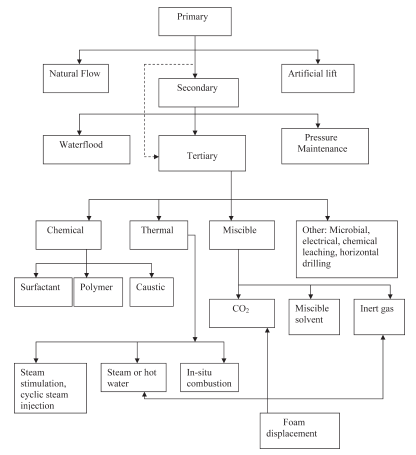
\includegraphics[width=.6\textwidth]{figs/revisao/revisao_recmethods}
	\caption{Resumo dos m\'{e}todos convencionais de recupera\c{c}\~{a}o \cite{adeniyi2008} \label{fig:recreview}}
\end{figure}

\subsection{M\'{e}todos Convencionais}
Os dois tipos de m\'{e}todos considerados convencionais, j\'{a} citados, s\~{a}o os m\'{e}todos de inje\c{c}\~{a}o imisc\'{i}vel de fluidos no reservat\'{o}rio, seja \'{a}gua ou g\'{a}s. Segundo Eremin, o m\'{e}todo de inje\c{c}\~{a}o de \'{a}gua \'{e} um dos mais utilizados devido \`{a} sua utiliza\c{c}\~{a}o tamb\'{e}m como m\'{e}todo mantenedor da press\~{a}o no reservat\'{o}rio, al\'{e}m do fato da \'{a}gua ser um fluido acess\'{i}vel, consideravelmente barato e possuir propriedade de deslocamento espec\'{i}fica \cite{eremin}. J\'{a} a inje\c{c}\~{a}o de imisc\'{i}vel de g\'{a}s consiste em inje\c{c}\~{a}o de fluido gasoso, mas de forma que ele n\~{a}o se misture ao \'{o}leo, criando uma mistura bif\'{a}sica \cite[p. 564]{engres}.

O uso de m\'{e}todos convencionais, como o de inje\c{c}\~{a}o de \'{a}gua, \'{e} antigo dentro da hist\'{o}ria da explora\c{c}\~{a}o do petr\'{o}leo; se considera que o primeiro caso de inje\c{c}\~{a}o de \'{a}gua ocorreu acidentalmente na Pensilv\^{a}nia, em 1865. Em 1880, se descobriu que a \'{a}gua, ao invadir os po\c{c}os por meio de areias rasas, contribu\'{i}a para um aumento na recupera\c{c}\~{a}o de \'{o}leo. Muitas das primeiras ocorr\^{e}ncias de invas\~{a}o de \'{a}gua nos reservat\'{o}rios eram acidentais, decorrentes de \'{a}guas provenientes de areias \'{u}midas ou da superf\'{i}cie invadindo os po\c{c}os e, consequentemente, o reservat\'{o}rio \cite{adeniyi2008}. A partir de 1950, afirmam Singh e Kiel, as t\'{e}cnicas de inje\c{c}\~{a}o de \'{a}gua se tornaram mais populares, sua utiliza\c{c}\~{a}o incrementando rapidamente. Atualmente, a inje\c{c}\~{a}o de \'{a}gua \'{e} ainda considerada como um dos m\'{e}todos de recupera\c{c}\~{a}o mais confi\'{a}veis e econ\^{o}micos, a ponto de se tornar a alternativa a ser usada em caso de deple\c{c}\~{a}o de reservat\'{o}rios cujo mecanismo \'{e} o influxo de \'{a}gua \cite{singh1982}.

Segundo Rosa, ao se escolher um projeto de inje\c{c}\~{a}o, deve-se levar em conta a escolha do esquema de inje\c{c}\~{a}o, isto \'{e}, da distribui\c{c}\~{a}o dos po\c{c}os de inje\c{c}\~{a}o e de produ\c{c}\~{a}o mais adequada ao reservat\'{o}rio de petr\'{o}leo em estudo. Como o objetivo primordial da inje\c{c}\~{a}o \'{e} o aumento da recupera\c{c}\~{a}o de petr\'{o}leo, deve-se tentar produzir esse volume adicional desejado utilizando-se esquemas em que os volumes de fluidos injetados sejam os menores poss\'{i}veis e a produ\c{c}\~{a}o do fluido injetado seja a menor poss\'{i}vel. Por fim, devem ser observadas as caracter\'{i}sticas particulares do reservat\'{o}rio em estudo, como a exist\^{e}ncia de falhas, varia\c{c}\~{o}es de permeabilidade, etc., al\'{e}m do aspecto econ\^{o}mico da produ\c{c}\~{a}o \cite[p. 564]{engres}; o aspecto econ\^{o}mico envolve estudo de custos relacionados \`{a} ado\c{c}\~{a}o do m\'{e}todo de recupera\c{c}\~{a}o, como os custos de estudo, de perfura\c{c}\~{a}o de novos po\c{c}os, da convers\~{a}o de po\c{c}os produtores em injetores, entre outros \cite{latil}.

De acordo com Latil, entre os m\'{e}todos convencionais de inje\c{c}\~{a}o de fluidos, o de inje\c{c}\~{a}o de g\'{a}s \'{e} mais indicado em casos de reservat\'{o}rios com baixa raz\~{a}o g\'{a}s-\'{o}leo --- neste caso, seria necess\'{a}ria um grande volume de g\'{a}s injetado para se criar a fase gasosa --- ou de \'{o}leo saturado, desde que a permeabilidade \`{a} \'{a}gua seja suficientemente alta; j\'{a} em casos de reservat\'{o}rios com alta raz\~{a}o gas-\'{o}leo, a inje\c{c}\~{a}o imisc\'{i}vel de g\'{a}s se torna um m\'{e}todo que resulta em melhores \'{i}ndices de recupera\c{c}\~{a}o de \'{o}leo. Por fim, em casos de reservat\'{o}rios heterog\^{e}neos com presen\c{c}a de \'{a}gua, a inje\c{c}\~{a}o de \'{a}gua \'{e} a mais recomendada \cite{latil}. 

\subsection{Esquemas de Inje\c{c}\~{a}o}

Ao se considerar o uso de t\'{e}cnicas de recupera\c{c}\~{a}o secund\'{a}ria, baseadas na inje\c{c}\~{a}o de fluidos, a efici\^{e}ncia do m\'{e}todo utilizado depende da maneira com que os po\c{c}os injetores e produtores s\~{a}o posicionados. A disposi\c{c}\~{a}o dos mesmos no reservat\'{o}rio deve ser tal que minimize o n\'{u}mero de po\c{c}os, mas maximizando a inje\c{c}\~{a}o de fluido e melhorando a recupera\c{c}\~{a}o de \'{o}leo \cite{dake}. O posicionamento dos po\c{c}os pode ser encarado como um \textit{esquema de inje\c{c}\~{a}o}. Segundo Rosa, h\'{a} v\'{a}rios tipos de esquemas de inje\c{c}\~{a}o, separados em dois grupos principais: os esquemas baseados na estrutura do reservat\'{o}rio (inje\c{c}\~{a}o perif\'{e}rica, no topo ou na base) ou baseados no modo como os po\c{c}os s\~{a}o distribu\'{i}dos (esquemas em malha) \cite[p. 564]{engres}.

\subsubsection{Esquemas baseados na Estrutura do Reservat\'{o}rio}
Nos esquemas baseados na estrutura do reservat\'{o}rio, os po\c{c}os de mesmo tipo (de inje\c{c}\~{a}o ou de produ\c{c}\~{a}o) se concentram em determinadas \'{a}reas do reservat\'{o}rio. Em reservat\'{o}rios de estrutura anticlinal, por exemplo, \'{e} mais utilizado o esquema de \textit{inje\c{c}\~{a}o perif\'{e}rica}, em que os po\c{c}os produtores se concentram no centro do reservat\'{o}rio, equanto que os injetores s\~{a}o situados na periferia do mesmo, justificando o nome do esquema\footnote{Ver \cite[p. 565]{engres}}. O esquema de inje\c{c}\~{a}o perif\'{e}rica pode ser aplicado juntamente com projetos de otimiza\c{c}\~{a}o dos injetores, como por exemplo o problema real abordado por Feng \textit{et al.}, tratando-se de um problema de \textit{design} de um projeto \'{o}timo de inje\c{c}\~{a}o de \'{a}gua em um campo de petr\'{o}leo situado no Equador \cite{feng2015}. 

A \textit{inje\c{c}\~{a}o no topo} consiste em situar os po\c{c}os injetores no topo do reservat\'{o}rio, enquanto os produtores s\~{a}o localizados na base; o fluido injetado, neste caso, \'{e} o g\'{a}s. Por fim, a \textit{inje\c{c}\~{a}o na base} considera os po\c{c}os injetores na base do reservat\'{o}rio e os produtores no topo, com a \'{a}gua sendo o fluido injetado. Vale notar que os esquemas de inje\c{c}\~{a}o no topo e na base podem ser combinados, e que, em determinado momento, os po\c{c}os produtores podem ser convertidos em po\c{c}os injetores. Rosa ainda destaca que, na verdade, essas diferentes maneiras de se fazer inje\c{c}\~{a}o n\~{a}o se classificam exatamente como
\textit{esquemas} de inje\c{c}\~{a}o, uma vez que a disposi\c{c}\~{a}o dos po\c{c}os n\~{a}o est\'{a} previamente estabelecida, ou seja, n\~{a}o existem arranjos prefixados para a localiza\c{c}\~{a}o dos po\c{c}os \cite[p. 566]{engres}.


Um fato a ser considerado com a inje\c{c}\~{a}o de \'{a}gua, afirma Patacchini, \'{e} que n\~{a}o \'{e} poss\'{i}vel simplemente adicionar a referida vari\'{a}vel \`{a}s equa\c{c}\~{o}es de balan\c{c}o de materiais em projetos de inje\c{c}\~{a}o perif\'{e}rica, uma vez que as equa\c{c}\~{o}es n\~{a}o consideram o volume de \'{a}gua perdido para o aqu\'{i}fero nem o tempo requerido para a difus\~{a}o da press\~{a}o para a borda do reservat\'{o}rio; contudo, o autor apresenta um m\'{e}todo que n\~{a}o s\'{o} contorna o problema apresentado como tamb\'{e}m consegue fazer com que a press\~{a}o do reservat\'{o}rio n\~{a}o dependa da efici\^{e}ncia dos injetores perif\'{e}ricos, e a vaz\~{a}o de inje\c{c}\~{a}o de \'{a}gua n\~{a}o afete o suporte do aqu\'{i}fero \cite{PATACCHINI2017720}.

\subsubsection{Esquemas de Inje\c{c}\~{a}o em Malha}
Neste grupo, se situam esquema de inje\c{c}\~{a}o aplicados em reservat\'{o}rios com grandes \'{a}reas e pequenas inclina\c{c}\~{o}es e espessuras; os po\c{c}os tanto de um tipo quanto do outro est\~{a}o uniformemente distribu\'{i}dos em toda a \'{a}rea do reservat\'{o}rio. Neste caso, o fluido deslocante \'{e} injetado na pr\'{o}pria zona de \'{o}leo, alterando-se drasticamente a distribui\c{c}\~{a}o de satura\c{c}\~{o}es e a movimenta\c{c}\~{a}o natural dos fluidos no reservat\'{o}rio \cite[p. 567]{engres}.

Dos tipos de inje\c{c}\~{a}o em malha, destacam-se as inje\c{c}\~{o}es em \textit{linha direta} e em \textit{linhas esconsas}, em que, os po\c{c}os de produ\c{c}\~{a}o e inje\c{c}\~{a}o s\~{a}o alternados em linhas, formando malhas normalmente retangulares; no caso das linhas esconsas, h\'{a} uma defasagem entre as linhas de produtores e injetores. As Figuras \ref{fig:rev_injld} e \ref{fig:rev_injle} mostram, respectivamente, exemplos de esquemas de linha direta e linhas esconsas.

\begin{figure}[!ht]
\centering
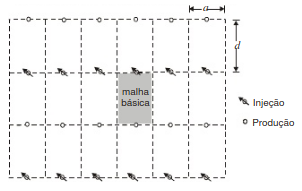
\includegraphics[width=.6\textwidth]{figs/revisao/revisao_injld.png}
\caption{Inje\c{c}\~{a}o em linha direta \cite[p. 567]{engres}.}
\label{fig:rev_injld}
\end{figure}

\begin{figure}[!ht]
\centering
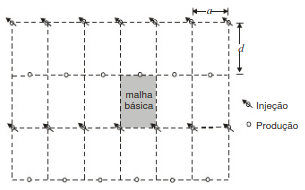
\includegraphics[width=.6\textwidth]{figs/revisao/revisao_injle.png}
\caption{Inje\c{c}\~{a}o em linhas esconsas \cite[p. 567]{engres}.}
\label{fig:rev_injle}
\end{figure}

Em alguns casos, os esquemas de malha em linhas diretas ou esconsas podem ser adaptados utilizando-se pol\'{i}gonos regulares como constituintes da malha; tr\^{e}s exemplos deste tipo de caso s\~{a}o:
\begin{itemize}
\item \textbf{Malha \textit{five-spot}:} Neste caso, a malha \'{e} formada por linhas esconsas, formando um quadrado perfeito; um po\c{c}o produtor \'{e} cercado por quatro injetores.
\item \textbf{Malha \textit{seven-spot}:} A malha considerada consiste em hex\'{a}gonos regulares, em que um po\c{c}o produtor \'{e} cercado por seis injetores; pode ser considerada um esquema de linhas esconsas, mas com altern\^{a}ncia de dois injetores para cada produtor em cada linha.
\item \textbf{Malha \textit{nine-spot}:} Assim como a malha \textit{five-spot}, \'{e} constitu\'{i}da por quadrados; por\'{e}m, o esquema de inje\c{c}\~{a}o base pode ser visto como linhas diretas, em que h\'{a} linhas s\'{o} de injetores e linhas alternadas entre produtores e injetores; neste tipo de malha, cada po\c{c}o produtor \'{e} cercado por oito po\c{c}os injetores.
\end{itemize}

Os esquemas de inje\c{c}\~{a}o em malhas vistos at\'{e} aqui consideram um po\c{c}o produtor cercado de v\'{a}rios injetores; s\~{a}o consideradas, portanto, malhas de tipo \textit{normal}. Contudo, as mesmas malhas podem tamb\'{e}m ser projetadas tomando-se em conta um po\c{c}o injetor cercado por v\'{a}rios produtores; s\~{a}o as chamadas \textit{malhas invertidas} ou \textit{inversas} \cite[p. 569]{engres}. A Figuras \ref{fig:rev_inj7i} mostra alguns exemplos de malhas de inje\c{c}\~{a}o, enquanto que a Tabela \ref{tab:wfdpat} destaca algumas informa\c{c}\~{o}es relativas aos esquemas de inje\c{c}\~{a}o vistos.

\begin{figure}[!ht]
\centering
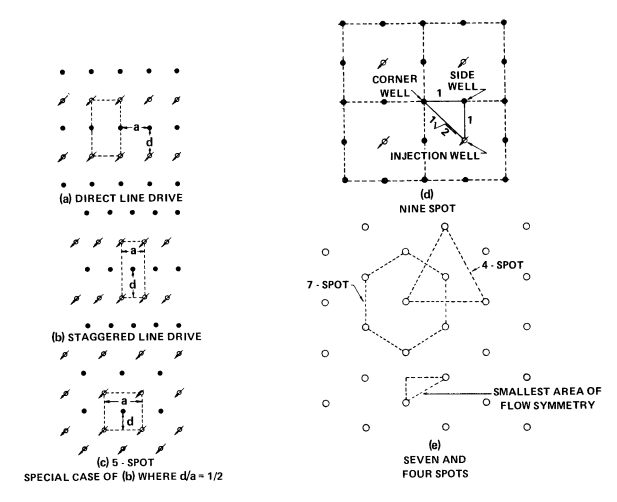
\includegraphics[width=.7\textwidth]{figs/revisao/revisao_injmalhas.png}
\caption{Exemplos de malhas de inje\c{c}\~{a}o \cite{singh1982}.}
\label{fig:rev_inj7i}
\end{figure}

\begin{table}[!ht]
	\centering
	\caption{Caracter\'{i}sticas de alguns esquemas de inje\c{c}\~{a}o, adaptado de \cite{singh1982}\label{tab:wfdpat}}
	\begin{tabular}{|c|c|c|}
		\hline
		\textbf{Esquema} & \textbf{Raz\~{a}o produtores/injetores} & \textbf{Padr\~{a}o de fura\c{c}\~{a}o} \\ \hline
		\textit{Four-spot} & $2$ & Tri\^{a}ngulo equil\'{a}tero \\ \hline
		\textit{Four-spot} obl\'{i}quo & $2$ & Quadrado \\ \hline
		\textit{Five-spot} & $1$ & Quadrado \\ \hline
		\textit{Seven-spot} & $\frac{1}{2}$ & Tri\^{a}ngulo equil\'{a}tero \\ \hline
		\textit{Seven-spot} invertido (injetor \'{u}nico) & $2$ & Tri\^{a}ngulo Equil\'{a}tero \\ \hline
		\textit{Nine-spot} & $\frac{1}{3}$ & Quadrado \\ \hline
		\textit{Nine-spot} invertido (injetor \'{u}nico) & $3$ & Quadrado \\ \hline
		Linhas diretas & $1$ & Ret\^{a}ngulo \\ \hline
		Linhas esconsas & $1$ & Linhas deslocadas \\ \hline
		
	\end{tabular}
\end{table}

Assim como no caso da inje\c{c}\~{a}o perif\'{e}rica, os esquemas de inje\c{c}\~{a}o em malhas possuem larga utiliza\c{c}\~{a}o na engenharia de reservat\'{o}rios; Zakirov \textit{et al.}, por exemplo, fazem a compara\c{c}\~{a}o de v\'{a}rios esquemas de malha no projeto de inje\c{c}\~{a}o de \'{a}gua no campo de Russkoye, situado acima do C\'{i}rculo Polar na R\'{u}ssia, com a an\'{a}lise feita em termos econ\^{o}micos e avalia\c{c}\~{a}o t\'{e}cnica \cite{zakirov2012}. Um outro uso \'{e} proposto por Zhou \textit{et al.}; por\'{e}m, neste caso os esquemas de inje\c{c}\~{a}o em malhas s\~{a}o testados em outros m\'{e}todos de recupera\c{c}\~{a}o, como a inje\c{c}\~{a}o de pol\'{i}meros e surfactantes \cite{zhou2016}.

\subsection{Aspectos Operacionais da Inje\c{c}\~{a}o de \'{A}gua}

O m\'{e}todo de recupera\c{c}\~{a}o secund\'{a}ria por inje\c{c}\~{a}o de \'{a}gua \'{e} ainda um dos mais utilizados; ela tem o objetivo de deslocar o \'{o}leo em dire\c{c}\~{a}o aos po\c{c}os produtores, aumentando assim a produ\c{c}\~{a}o de petr\'{o}leo em rela\c{c}\~{a}o \`{a} recupera\c{c}\~{a}o prim\'{a}ria.

A inje\c{c}\~{a}o de \'{a}gua no reservat\'{o}rio faz com que a satura\c{c}\~{a}o de \'{a}gua se eleve nas imedia\c{c}\~{o}es dos po\c{c}os injetores; esse aumento de satura\c{c}\~{a}o gera um banco de \'{o}leo cujo avan\c{c}o se d\'{a} em dire\c{c}\~{a}o aos po\c{c}os produtores. Uma vez alcan\c{c}ando esses po\c{c}os, o banco de \'{o}leo faz com que a produ\c{c}\~{a}o de \'{o}leo aumente bruscamente. 

Segundo Rosa, o per\'{i}odo de tempo entre o in\'{i}cio das opera\c{c}\~{o}es e a chegada do \'{o}leo ao po\c{c}o produtor \'{e} chamado de tempo de enchimento (\textit{``fill up''}); posteriormente, a frente de avan\c{c}o atinge o po\c{c}o produtor, aumentando bruscamente a raz\~{a}o \'{a}gua/\'{o}leo (RAO), ocorrendo ent\~{a}o o que se chama de erup\c{c}\~{a}o (\textit{``breakthrough''}). Ap\'{o}s a erup\c{c}\~{a}o, a RAO continua a crescer at\'{e} atingir n\'{i}veis que ir\~{a}o inviabilizar economicamente a produ\c{c}\~{a}o do po\c{c}o, o qual \'{e} fechado ou eventualmente transformado em po\c{c}o injetor \cite{engres}.

\subsubsection{Fatores de Influ\^{e}ncia}

Os projetos de inje\c{c}\~{a}o de \'{a}gua dependem n\~{a}o somente do objetivo de se obter uma melhor produ\c{c}\~{a}o de petr\'{o}leo; os fatores f\'{i}sicos do reservat\'{o}rio, por exemplo, tamb\'{e}m devem ser levados em conta na fase inicial do projeto. Os seguintes fatores ajudam a ditar par\^{a}metros de um projeto de inje\c{c}\~{a}o de \'{a}gua\footnote{Ver \cite[pp. 652-653]{engres}} (como formato da malha de inje\c{c}\~{a}o, n\'{u}mero de injetores, entre outros):

\begin{enumerate}
\item \textbf{Mecanismos de produ\c{c}\~{a}o do reservat\'{o}rio:} A depender do mecanismo de produ\c{c}\~{a}o, a quantidade de \'{a}gua a ser injetada varia; no caso de um influxo de \'{a}gua, por exemplo, ser\'{a} requerida uma menor vaz\~{a}o de inje\c{c}\~{a}o (ou essa vaz\~{a}o at\'{e} poder\'{a} ser nula) para que a press\~{a}o do reservat\'{o}rio seja mantida. O balan\c{c}o de materiais (diferen\c{c}a entre o volume que sai e o volume que \'{e} reposto pela natureza) ir\'{a} determinar o volume e a vaz\~{a}o total que dever\'{a} ser reposta pela recupera\c{c}\~{a}o secund\'{a}ria. J\'{a} no caso do mecanismo de g\'{a}s em solu\c{c}\~{a}o, a quantidade de \'{a}gua injetada deve ser maior, pois a press\~{a}o tende a cair rapidamente, ou seja, a deple\c{c}\~{a}o do reservat\'{o}rio \'{e} mais r\'{a}pida, acarretando urg\^{e}ncia na ado\c{c}\~{a}o da recupera\c{c}\~{a}o secund\'{a}ria.

\item \textbf{Caracter\'{i}sticas da rocha:} Caracter\'{i}sticas como permeabilidade, porosidade, presen\c{c}a de finos, a argila do reservat\'{o}rio e sua composi\c{c}\~{a}o qu\'{i}mica s\~{a}o determinantes em um projeto de inje\c{c}\~{a}o de \'{a}gua; de acordo com Eremin e Nazarova, por exemplo, caso haja uma incompatibilidade qu\'{i}mica entre a \'{a}gua injetada e o reservat\'{o}rio, haver\'{a} uma deposi\c{c}\~{a}o de sais que, consequentemente, afetam a pososidade e a permeabilidade do reservat\'{o}rio, reduzindo a recupera\c{c}\~{a}o de \'{o}leo nos po\c{c}os produtores \cite{eremin}.

\item \textbf{Caracter\'{i}sticas dos fluidos:} Assim como nas caracter\'{i}sticas da rocha, deve-se haver uma compatibilidade qu\'{i}mica entre a \'{a}gua injetada e os fluidos do reservat\'{o}rio, de maneira a evitar a forma\c{c}\~{a}o de precipitados; al\'{e}m disso, caso haja uma alta raz\~{a}o de mobilidades entre o \'{o}leo e a \'{a}gua, deve-se aumentar o n\'{u}mero de po\c{c}os injetores e diminuir a vaz\~{a}o dos mesmos, de maneira a evitar um \textit{``breakthrough''} prematuro nos po\c{c}os produtores.

\item \textbf{Profundidade do reservat\'{o}rio:} O gradiente m\'{a}ximo de press\~{a}o entre os po\c{c}os injetores e o reservat\'{o}rio \'{e} diretamente influenciado pela sua profundidade, por esta ser proporcional \`{a}s press\~{o}es de inje\c{c}\~{a}o e fraturamento do reservat\'{o}rio.

\item \textbf{Conforma\c{c}\~{a}o estrutural do reservat\'{o}rio:} A depender da estrutura do reservat\'{o}rio, torna-se preferencial a ado\c{c}\~{a}o de esquemas de inje\c{c}\~{a}o espec\'{i}ficos; o esquema de inje\c{c}\~{a}o perif\'{e}rica, por exemplo, \'{e} adequado para reservat\'{o}rios muito inclinados, onde a segrega\c{c}\~{a}o gravitacional dos fluidos \'{e} grande.
\end{enumerate}

Os fatores de influ\^{e}ncia, al\'{e}m de ditar o n\'{u}mero de injetores e a vaz\~{a}o de inje\c{c}\~{a}o, por exemplo, tamb\'{e}m s\~{a}o determinantes para a escolha do esquema de inje\c{c}\~{a}o a ser adotado, conforme afirma Stephens; o autor cita exemplos de reservat\'{o}rios em que, por exemplo, \'{e} invi\'{a}vel a ado\c{c}\~{a}o de projetos de inje\c{c}\~{a}o em malha, como o \textit{five-spot}, e outros em que n\~{a}o \'{e} recomendado o uso de inje\c{c}\~{a}o perif\'{e}rica; no seu trabalho, Stephens cita cinco exemplos de casos baseados em reservat\'{o}rios reais, discutindo qual o melhor esquema de inje\c{c}\~{a}o para os mesmos, considerando-se os par\^{a}metros dos reservat\'{o}rios \cite{stephens1960}.

\subsubsection{Componentes Principais de um Sistema de Inje\c{c}\~{a}o}

Vistos os fatores que influenciam um projeto de recupera\c{c}\~{a}o secund\'{a}ria por inje\c{c}\~{a}o de \'{a}gua, procede-se \`{a} descri\c{c}\~{a}o dos seus componentes principais\footnote{Ver \cite[pp. 653-659]{engres}}:

\begin{enumerate}
\item \textbf{Capta\c{c}\~{a}o:} A capta\c{c}\~{a}o do fluido injetado pode se dar de rios, lagos, mares, subsuperf\'{i}cie, \'{a}gua de produ\c{c}\~{a}o ou at\'{e} mesmo de outros campos de reservat\'{o}rios.

\item \textbf{Adu\c{c}\~{a}o:} Sistema de transporte \'{a}gua. Como lida com \'{a}gua n\~{a}o tratada, devem ser empregados materiais resistentes \`{a} agressividade da \'{a}gua para desenvolver esse sistemas. A redu\c{c}\~{a}o de dep\'{o}sitos s\'{o}lidos tamb\'{e}m deve ser considerada.

\item \textbf{Tancagem:} Sistema de armazenamento de \'{a}gua; a depender do tipo de capta\c{c}\~{a}o da \'{a}gua, a tancagem de \'{a}gua bruta pode ser largamente utilizada ou at\'{e} mesmo dispensada (como em casos de capta\c{c}\~{a}o da \'{a}gua do mar). A tancagem de \'{a}gua pot\'{a}vel, por outro lado, \'{e} necess\'{a}ria para armazenar reserva para determinados equipamentos, como por exempo, \'{a}gua limpa para contra-lavagem dos filtros ou para refrigera\c{c}\~{a}o de bombas.

\item \textbf{Tratamento:} A \'{a}gua bruta a ser utilizada precisa ser tratada, de maneira a ser propriamente injetada; os dois principais m\'{e}todos utilizados de tratamento s\~{a}o a retirada de s\'{o}lidos e o controle bacteriol\'{o}gico, j\'{a} que as bact\'{e}rias tendem a consumir o petr\'{o}leo, por este ser composto majoritariamente de mat\'{e}ria org\^{a}nica.

\item \textbf{Conjunto motor-bomba:} Respons\'{a}vel pelo fornecimento de energia para a \'{a}gua se deslocar em dire\c{c}\~{a}o ao reservat\'{o}rio com a vaz\~{a}o desejada. Dois tipos de bombas s\~{a}o normalmente utilizados: bombas centr\'{i}fugas, em sistemas de press\~{a}o mais baixa, e bombas alternativas (deslocamento positivo) em sistemas de alta press\~{a}o.

\item \textbf{Rede de distribui\c{c}\~{a}o:} Integra a esta\c{c}\~{a}o de inje\c{c}\~{a}o de \'{a}gua, um sistema adutor e os po\c{c}os de inje\c{c}\~{a}o. H\'{a} dois tipos, apresentados na Figura \ref{fig:rev_redis}: a rede de distribui\c{c}\~{a}o em marcha (``espinha de peixe'') e a centralizada atrav\'{e}s de \textit{``manifolds''} (``p\'{e} de galinha'').

\begin{figure}[!ht]
\centering
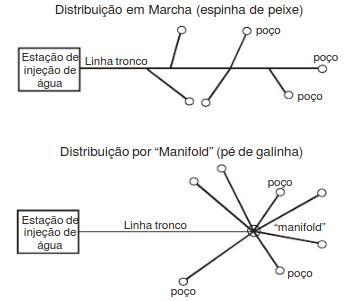
\includegraphics[width=.6\textwidth]{figs/revisao/revisao_redis.png}
\caption{Esquemas de redes de distribui\c{c}\~{a}o \cite[p. 657]{engres}.}\label{fig:rev_redis}
\end{figure}

\item \textbf{Po\c{c}os de inje\c{c}\~{a}o:} A maioria dos po\c{c}os injetores s\~{a}o, na verdade, antigos po\c{c}os produtores convertidos ou recompletados para inje\c{c}\~{a}o; h\'{a} at\'{e} mesmo casos em que o mesmo po\c{c}o comporta uma zona produtora e outra injetora. Alguns tipos de completa\c{c}\~{a}o de po\c{c}os injetores s\~{a}o apresentados na Figura \ref{fig:rev_incmp}. 

\begin{figure}[!ht]
\centering
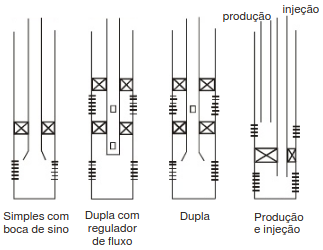
\includegraphics[width=.6\textwidth]{figs/revisao/revisao_injcomp.png}
\caption{Tipos de completa\c{c}\~{a}o de po\c{c}os de inje\c{c}\~{a}o de \'{a}gua \cite[p. 658]{engres}.}\label{fig:rev_incmp}
\end{figure}

\item \textbf{Po\c{c}os de capta\c{c}\~{a}o:} Normalmente, s\~{a}o antigos po\c{c}os produtores de \'{o}leo, recompletados (recanhoneados) em zonas produtoras de \'{a}gua. Apesar de serem po\c{c}os previamente abandonados, s\~{a}o po\c{c}os problem\'{a}ticos, devido \`{a}s altas vaz\~{o}es de fluido com sais dissolvidos, tais po\c{c}os produzem areia, diminuindo a vida \'{u}til dos equipamentos.

\item \textbf{Po\c{c}os de \textit{``dump-flood''}:} S\~{a}o os sistemas mais simples de inje\c{c}\~{a}o de \'{a}gua, consistindo simplesmente em po\c{c}os simultaneamente produtores e injetores de \'{a}gua, isto \'{e}, produzem \'{a}gua na zona superior e injetam diretamente, por gravidade, na zona inferior. A opera\c{c}\~{a}o desse tipo de po\c{c}o \'{e} muito simples, mas o acompanhamento somente \'{e} poss\'{i}vel atrav\'{e}s de perfilagens peri\'{o}dicas com o chamado
medidor de fluxo cont\'{i}nuo (\textit{``continuous flow meter''}) ou com perfilagem radiativa.
\end{enumerate}

\'{E} importante destacar a necessidade de se ter aten\c{c}\~{a}o \`{a}s caracter\'{i}sticas dos po\c{c}os de inje\c{c}\~{a}o projetados de maneira a se obter o desempenho \'{o}timo; Palsson \textit{et al.} citam algumas dessas caracter\'{i}sticas, como inclina\c{c}\~{a}o e orienta\c{c}\~{a}o dos po\c{c}os, completa\c{c}\~{a}o e danos de perfura\c{c}\~{a}o e completa\c{c}\~{a}o. Os desafios t\'{e}cnicos principais s\~{a}o:

\begin{itemize}
	\item Obter e manter a vaz\~{a}o de inje\c{c}\~{a}o desejada;
	\item Controlar o perfil de injetividade para a obten\c{c}\~{a}o da m\'{a}xima efici\^{e}ncia de varrido;
	\item Reduzir as incertezas na opera\c{c}\~{a}o esperada da inje\c{c}\~{a}o nos po\c{c}os.
\end{itemize}

Os autores ainda destacam a import\^{a}ncia da completa\c{c}\~{a}o dos po\c{c}os de inje\c{c}\~{a}o com o intuito dos mesmos suportarem altas press\~{o}es de inje\c{c}\~{a}o e diminuir custos de manuten\c{c}\~{a}o, como troca de tubos; al\'{e}m disso, s\~{a}o citados alguns problemas que podem surgir durante projetos de inje\c{c}\~{a}o, como o caso da perda de po\c{c}os devido ao entupimento com areia, consequ\^{e}ncia da presen\c{c}a de po\c{c}os injetores em forma\c{c}\~{o}es n\~{a}o consolidadas \cite{PALSSON2003333}. 

\subsubsection{Controle e Acompanhamento}
De maneira a se acompanhar satisfatoriamente um projeto de inje\c{c}\~{a}o de \'{a}gua, n\~{a}o se deve apenas controlar os valores de vaz\~{a}o, mantendo-as nas cotas estabelecidas; tal controle, segundo Rosa, seria suficiente se as forma\c{c}\~{o}es fossem homog\^{e}neas e as suas condi\c{c}\~{o}es de permeabilidade e press\~{a}o se mantivessem inalteradas ao longo do tempo. Sabe-se, contudo, que isso \'{e} praticamente imposs\'{i}vel de ocorrer, devendo-se portanto realizar testes peri\'{o}dicos para que possam ser identificadas situa-\c{c}\~{o}es indesejadas como, por exemplo, dano \`{a} forma\c{c}\~{a}o e m\'{a} distribui\c{c}\~{a}o da \'{a}gua. Algumas estrat\'{e}gias de controle e acompanhamento s\~{a}o apresentadas a seguir\footnote{Ver \cite[pp. 659-662]{engres}}:

\begin{enumerate}
\item \textbf{Testes:} H\'{a} v\'{a}rios tipos de testes para acompanhamento dos po\c{c}os de inje\c{c}\~{a}o de \'{a}gua; entre eles o teste de inje\c{c}\~{a}o, que busca acompanhar a vaz\~{a}o e a press\~{a}o de inje\c{c}\~{a}o, fornecendo uma primeira ideia do comportamento do po\c{c}o; o teste de \textit{fall-off}, que avalia se a forma\c{c}\~{a}o est\'{a} danificada, estimulada ou se est\'{a} em sua condi\c{c}\~{a}o original; e o teste \textit{step rate}, que, ao realizar a inje\c{c}\~{a}o com press\~{o}es variadas, obt\'{e}m valores distintos de vaz\~{o}es; com esses dados, \'{e} poss\'{i}vel construir um gr\'{a}fico da vaz\~{a}o em fun\c{c}\~{a}o da press\~{a}o, conforme ilustra a Figura \ref{fig:rev_tst}.

\begin{figure}[!ht]
\centering
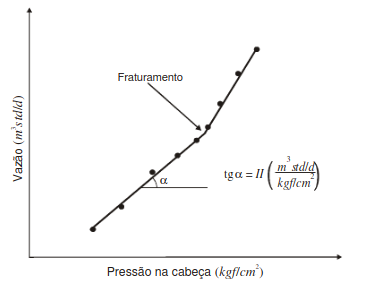
\includegraphics[width=.6\textwidth]{figs/revisao/revisao_tst.png}
\caption{Teste \textit{step rate} \cite[p. 660]{engres}.}\label{fig:rev_tst}
\end{figure}

\item \textbf{\'{I}ndice de injetividade:} Similar ao \'{i}ndice de produtividade para po\c{c}os produtores, esse \'{i}ndice pode indicar, se calculado periodicamente, a causa do decr\'{e}scimo de vaz\~{a}o durante os primeiros est\'{a}gios de inje\c{c}\~{a}o de um po\c{c}o; esse \'{i}ndice pode ser estimado a partir de testes de inje\c{c}\~{a}o, \textit{fall-off} ou \textit{step rate}.

\item \textbf{Perfil de Injetividade:} Destina-se \`{a} investiga\c{c}\~{a}o da distribui\c{c}\~{a}o de \'{a}gua atrav\'{e}s da forma\c{c}\~{a}o, uma vez que a presen\c{c}a de fraturas naturais ou induzidas, zonas de alta permeabilidade devidas \`{a} heterogeneidade do reservat\'{o}rio, etc., podem provocar uma erup\c{c}\~{a}o precoce de \'{a}gua de inje\c{c}\~{a}o nos po\c{c}os produtores, prejudicando a efici\^{e}ncia de varrido e, consequentemente, a produ\c{c}\~{a}o. Deste modo, com a corre\c{c}\~{a}o de eventuais anomalias, consegue-se aumentar a recupera\c{c}\~{a}o de \'{o}leo e reduzir a produ\c{c}\~{a}o de \'{a}gua, logo reduzindo-se os gastos com tratamento qu\'{i}mico, principalmente.
\end{enumerate} 

O processo de controle e acompanhamento de projetos de inje\c{c}\~{a}o de \'{a}gua se econtra bem difundido na literatura; Talash, por exemplo, afirma que um fator essencial para o sucesso de um projeto de inje\c{c}\~{a}o de \'{a}gua envolve um programa de controle e acompanhamento bem planejados e executados\footnote{O autor destaca m\'{e}todos de acompanhamento n\~{a}o s\'{o} do projeto de inje\c{c}\~{a}o, como o de reservat\'{o}rios e tamb\'{e}m dos componentes; ver \cite{talash1988}.}. J\'{a} Palsson \textit{et al.} consideram que o monitoramento da injetividade de \'{a}gua \'{e} comumente limitado a medidas de press\~{a}o e vaz\~{a}o em intervalos de tempo regulares; os autores citam algumas formas de apresenta\c{c}\~{a}o dos dados, como curvas de press\~{a}o/vaz\~{a}o, curvas de press\~{a}o e vaz\~{a}o em fun\c{c}\~{a}o do tempo, diagrama de Hall, entre outros; al\'{e}m disso, afirmam que essas representa\c{c}\~{o}es podem identificar mudan\c{c}as na injetividade dos po\c{c}os \cite{PALSSON2003333}.

\subsubsection{Principais Problemas}
Alguns dos principais problemas envolvendo a inje\c{c}\~{a}o de \'{a}gua s\~{a}o relacionados, al\'{e}m do aspecto econ\^{o}mico, tamb\'{e}m aos aspectos f\'{i}sico-qu\'{i}micos do fluido injetado e do reservat\'{o}rio. Um problema not\'{a}vel \'{e} a corros\~{a}o met\'{a}lica em sistemas de inje\c{c}\~{a}o, particularmente em casos de \'{a}guas com elevada salinidade e gases dissolvidos como oxig\^{e}nio, sulfeto de hidrog\^{e}nio e di\'{o}xido de carbono. Rosa apresenta alguns efeitos f\'{i}sicos-qu\'{i}micos diretamente relacionados ao fen\^{o}meno da corros\~{a}o met\'{a}lica \cite[pp. 662-663]{engres}:

\begin{enumerate}
\item \textbf{Efeitos da composi\c{c}\~{a}o da \'{a}gua:} Al\'{e}m da presen\c{c}a de gases dissolvidos ser um importante fator na corros\~{a}o met\'{a}lica, a pr\'{o}pria condutividade da \'{a}gua \'{e} diretamente proporcional \`{a} sua corrosividade.

\item \textbf{Efeitos de vari\'{a}veis f\'{i}sicas:} A temperatura, a press\~{a}o e a velocidade da \'{a}gua s\~{a}o fatores determinantes para sua corrosividade; a temperatura, por exemplo, aumenta drasticamente a corros\~{a}o quando elevada em sistemas fechados. Por\'{e}m, em sistemas abertos, a corros\~{a}o aumenta com a temperatura aumenta at\'{e} certo ponto, passando a diminuir por conta da libera\c{c}\~{a}o r\'{a}pida dos gases dissolvidos. A press\~{a}o \'{e} determinante para alterar rea\c{c}\~{o}es qu\'{i}micas; nos sistemas de inje\c{c}\~{a}o de \'{a}gua, ela influi diretamente na solubilidade dos gases em solu\c{c}\~{a}o, variando a taxa de corros\~{a}o. Por fim, a velocidade da \'{a}gua, ao ser elevada, acarreta em uma taxa de corros\~{a}o maior; por\'{e}m, \'{a}guas paradas ou de baixa vaz\~{a}o podem provocar a decanta\c{c}\~{a}o de s\'{o}lidos em suspens\~{a}o nos equipamentos de inje\c{c}\~{a}o.
\end{enumerate}

Um outro problema relevante em sistemas de inje\c{c}\~{a}o de \'{a}gua tem a ver com a forma\c{c}\~{a}o, devido aos componentes dissolvidos na \'{a}gua e outros fatores, de dep\'{o}sitos salinos nos equipamentos. Em quase todas as \'{a}guas, por exemplo, h\'{a} a presen\c{c}a de sais de c\'{a}lcio e magn\'{e}sio, cuja deposi\c{c}\~{a}o \'{e} a menos danosa, por ser facilmente remediada. J\'{a} a presen\c{c}a de compostos ferrosos conduzem \`{a} corros\~{a}o galv\^{a}nica; a presen\c{c}a de sulfetos \'{e} a mais danosa, pois, al\'{e}m da corros\~{a}o, provoca abras\~{a}o por atrito nas tubula\c{c}\~{o}es. Um outro efeito danoso dos sulfetos \'{e} a ocorr\^{e}ncia de s\'{e}rios danos \`{a} forma\c{c}\~{a}o, podendo ocasionar o tamponamento total da mesma.

Outros tipos de sais que se depositam nos sistemas de inje\c{c}\~{a}o de \'{a}gua e reservat\'{o}rios s\~{a}o os sais de b\'{a}rio. Estes causam danos \`{a} forma\c{c}\~{a}o irrevers\'{i}veis, pois o sulfato de b\'{a}rio, por exemplo, \'{e} insol\'{u}vel em \'{a}cidos, que normalmente s\~{a}o utilizados para lidar com dep\'{o}sitos salinos; neste caso, uma das medidas para evitar essa deposi\c{c}\~{a}o \'{e} impedir a forma\c{c}\~{a}o do sulfato de b\'{a}rio a partir do uso de inibidores qu\'{i}micos. Por fim, outro tipo de deposi\c{c}\~{a}o em sistemas de inje\c{c}\~{a}o \'{e} a s\'{i}lica, que, al\'{e}m de formar deposi\c{c}\~{o}es, pode auxiliar no tamponamento de linhas por outros precipitados ou at\'{e} mesmo ser aglutinada pelo \'{o}leo residual da \'{a}gua produzida. Neste caso, \'{e} empregado \'{a}cido fluor\'{i}drico para dissolv\^{e}-la\footnote{Todos esses problemas de deposi\c{c}\~{a}o de sais s\~{a}o explicados em \cite[p. 664]{engres}.}.

Outro problema a ser considerado considerando-se os fatores qu\'{i}micos envolvidos na inje\c{c}\~{a}o de \'{a}gua \'{e} a forma\c{c}\~{a}o de l\^{a}minas salinas nos tubos; segundo Adeniyi \textit{et al.}, esse fato acontece geralmente com a inje\c{c}\~{a}o de \'{a}gua n\~{a}o compat\'{i}vel com o reservat\'{o}rio, como por exemplo a inje\c{c}\~{a}o de \'{a}gua do mar em forma\c{c}\~{o}es ricas em \'{i}ons de estr\^{o}ncio e b\'{a}rio. Os autores citam os seguintes problemas potenciais\footnote{Ver \cite{adeniyi2008}}:

\begin{enumerate}
	\item O ato de elevar e tratar a \'{a}gua de inje\c{c}\~{a}o pode causar problemas uma vez que a \'{a}gua injetada se torna inst\'{a}vel, gerando um problema cont\'{i}nuo;
	\item Injetar uma \'{a}gua est\'{a}vel, por\'{e}m incompat\'{i}vel com o reservat\'{o}rio em um novo po\c{c}o injetor tamb\'{e}m pode causar a forma\c{c}\~{a}o de l\^{a}minas. Esse problema diminui gradativamente com a lavagem completa do po\c{c}o com a \'{a}gua de inje\c{c}\~{a}o.
\end{enumerate}

Al\'{e}m do problema da deposi\c{c}\~{a}o de l\^{a}minas salinas, Adeniyi \textit{et al.} tamb\'{e}m tratam do problema da corros\~{a}o; os autores afirmam que as principais causas de corros\~{a}o envolvem destrui\c{c}\~{a}o de ferro, e que esse problema \'{e} o que mais afeta, de maneira adversa, a produ\c{c}\~{a}o, o transporte e o refino; tal fato ocorre com a presen\c{c}a impurezas que geram c\'{e}lulas eletrol\'{i}ticas, aumentando a possibilidade de corros\~{a}o; a substitui\c{c}\~{a}o dessas impurezas por carbono, no processo de fabria\c{c}\~{a}o do a\c{c}o, \'{e} um modo de controlar esse problema \cite{adeniyi2008}.
%TCIDATA{LaTeXparent=0,0,cap_RevisaoBibliografica.tex}

\section{Simula\c{c}\~{a}o Num\'{e}rica de Reservat\'{o}rios}
\subsection{Vis\~{a}o Geral}
A simula\c{c}\~{a}o num\'{e}rica de um reservat\'{o}rio \'{e}, segundo Peaceman, \'{e} o processo de infer\^{e}ncia do comportamento do reservat\'{o}rio real dada a performance obtida de um modelo do mesmo, matem\'{a}tico ou f\'{i}sico (em escala laboratorial). Um modelo matem\'{a}tico de reservat\'{o}rio pode ser enxergado como um conjunto de equa\c{c}\~{o}es diferenciais parciais, juntamente com as condi\c{c}\~{o}es de contorno adequadas, que podem ser utilizadas para descrever satisfatoriamente os processos f\'{i}sicos importantes que ocorrem no sistema real. Os processos que ocorrem em um reservat\'{o}rio s\~{a}o basicamente transporte de fluidos e transfer\^{e}ncia de massa; at\'{e} tr\^{e}s fases imisc\'{i}veis (\'{o}leo, g\'{a}s e \'{a}gua) fluem simultaneamente, enquanto que o transporte de massa se d\'{a} entre as fases (notadamente entre o \'{o}leo e o g\'{a}s). A gravidade, a capilaridade e as for\c{c}as viscosas s\~{a}o tamb\'{e}m importantes no processo de vaz\~{a}o dos fluidos \cite{simres}.

Al\'{e}m da defini\c{c}\~{a}o proposta por Peaceman, Heimsund descreve a simula\c{c}\~{a}o de reservat\'{o}rios como uma ferramenta de investiga\c{c}\~{a}o da vaz\~{a}o de fluidos em subsuperf\'{i}cie. O autor destaca que as simula\c{c}\~{o}es de reservat\'{o}rio abrangem \'{a}reas relacionadas a ramos importantes da ci\^{e}ncia, como matem\'{a}tica, f\'{i}sica, qu\'{i}mica, geologia e biologia; al\'{e}m disso, afirma que, na ind\'{u}stria petrol\'{i}fera, os principais usos dos simuladores de reservat\'{o}rios envolvem a obten\c{c}\~{a}o de esquemas \'{o}timos de explota\c{c}\~{a}o e predi\c{c}\~{a}o da produ\c{c}\~{a}o\cite{heimsund2005}. J\'{a} Dake afirma que um simulador num\'{e}rico de reservat\'{o}rio \'{e} um programa de computador em que o sistema estudado \'{e} dividido em v\'{a}rias c\'{e}lulas discretas, cujas propriedades podem ser diferentes entre si \cite{dake}.

Segundo Rosa, a primeira etapa de uma simula\c{c}\~{a}o num\'{e}rica \'{e} formular o problema f\'{i}sico a ser representado matematicamente; em seguida s\~{a}o feitas suposi\c{c}\~{o}es e simplifica\c{c}\~{o}es compat\'{i}veis com o grau de sofistica\c{c}\~{a}o esperado do modelo, levando-se \`{a} formula\c{c}\~{a}o das equa\c{c}\~{o}es matem\'{a}ticas que descrevem o problema desejado, considerando-se as hip\'{o}teses adotadas. O passo seguinte \'{e} a resolu\c{c}\~{a}o das equa\c{c}\~{o}es e an\'{a}lise da solu\c{c}\~{a}o obtida; posteriormente, a validade do simulador \'{e} verificada atrav\'{e}s da calibra\c{c}\~{a}o com uma solu\c{c}\~{a}o existente --- por exemplo, comparam-se os resultados obtidos do simulador num\'{e}rico com solu\c{c}\~{o}es anal\'{i}ticas, resultados reais ou com resultados obtidos de modelos f\'{i}sicos de laborat\'{o}rio (dados experimentais). Caso o simulador seja considerado v\'{a}lido, o mesmo estar\'{a} pronto para ser utilizado na simula\c{c}\~{a}o do fen\^{o}meno desejado; caso contr\'{a}rio, volta-se para um novo ciclo em que s\~{a}o revistas as hip\'{o}teses adotadas ou at\'{e} a conceitua\c{c}\~{a}o do modelo f\'{i}sico \cite[p. 520]{engres}. A Figura \ref{fig:rev_simuesq} esquematiza um desenvolvimento b\'{a}sico de um simulador num\'{e}rico qualquer, enquanto que a Figura \ref{fig:rev_simuex} mostra uma compara\c{c}\~{a}o de resultados entre diferentes simuladores existentes, exemplificando o uso da calibra\c{c}\~{a}o com solu\c{c}\~{o}es j\'{a} obtidas para se validar um simulador de reservat\'{o}rio. 

\begin{figure}[H]
\centering
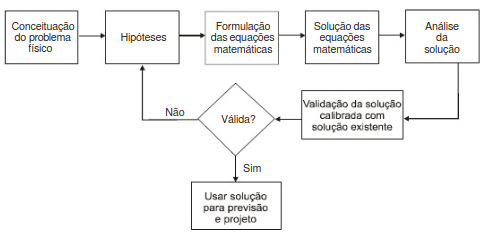
\includegraphics[width=.75\textwidth]{figs/revisao/revisao_simuesq.png}
\caption{Esquema b\'{a}sico de desenvolvimento de um simulador num\'{e}rico de reservat\'{o}rio \cite[p. 519]{engres}.}\label{fig:rev_simuesq}
\end{figure}

\begin{figure}[H]
\centering
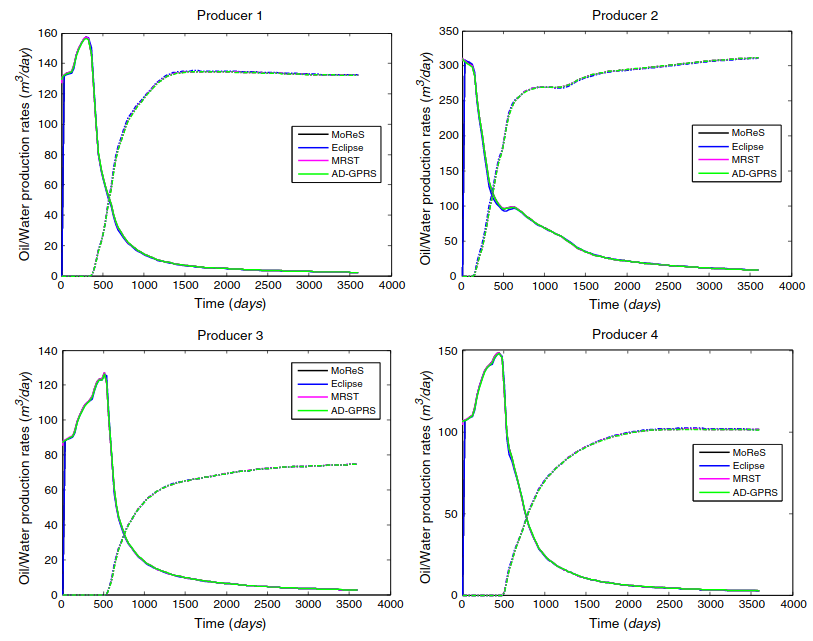
\includegraphics[width=.75\textwidth]{figs/revisao/revisao_simuex.png}
\caption{Exemplo de compara\c{c}\~{a}o de dados entre simuladores de vaz\~{a}o de \'{a}gua e de \'{o}leo de um modelo \cite{eggM}.}\label{fig:rev_simuex}
\end{figure}

\subsection{Hist\'{o}ria da Simula\c{c}\~{a}o de Reservat\'{o}rios}
Para se tra\c{c}ar a evolu\c{c}\~{a}o da simula\c{c}\~{a}o de reservat\'{o}rios ao longo da hist\'{o}ria, consideram-se aqui, inicialmente, fatos apresentados por Coats e por Breitenbach; de acordo com Coats, a simula\c{c}\~{a}o de reservat\'{o}rios \'{e} praticada desde o surgimento da engenharia de petr\'{o}leo, durante a d\'{e}cada de 1930. J\'{a} na d\'{e}cada de 1940, segundo Breitenbach, a simula\c{c}\~{a}o de reservat\'{o}rios passa a ser reconhecida, com as companhias desenvolvendo m\'{e}todos anal\'{i}ticos e num\'{e}ricos para a melhoria das solu\c{c}\~{o}es anal\'{i}ticas resistentes, balan\c{c}o de materiais e c\'{a}lculo de posicionamento 1-D de Buckley-Leverett; na d\'{e}cada seguinte (1950), as pesquisas por solu\c{c}\~{o}es num\'{e}ricas das equa\c{c}\~{o}es de vaz\~{a}o come\c{c}am a surtir efeito, com o surgimento de programas computacionais rudimentares, por\'{e}m eficientes, de simula\c{c}\~{o}es de reservat\'{o}rios. Considera-se um grande avan\c{c}o o surgimento dessas solu\c{c}\~{o}es, em que foi poss\'{i}vel resolver equa\c{c}\~{o}es de diferen\c{c}as finitas em modelos 2D e 3D, al\'{e}m de simula\c{c}\~{o}es em meios de porosidade heterog\^{e}nea; enfim, problemas mais complexos de engenharia de reservat\'{o}rio podiam ser resolvidos\footnote{Ver \cite{coats1982} e \cite{breitenbach1991}}.

A d\'{e}cada de 1960 representou, segundo Coats, um marco importante, em que a palavra ``simula\c{c}\~{a}o'' se torna comum, \`{a} medida em que os programas destinados \`{a} resolu\c{c}\~{a}o de problemas de reservat\'{o}rios se tornavam mais sofisticados; durante essa d\'{e}cada, os esfor\c{c}os na busca de simuladores melhores de reservat\'{o}rios se concentraram em modelos bif\'{a}sicos de g\'{a}s/\'{a}gua e \textit{black-oil} trif\'{a}sicos; os m\'{e}todos de recupera\c{c}\~{a}o de \'{o}leo simulados se restringiam essencialmente \`{a} deple\c{c}\~{a}o ou manuten\c{c}\~{a}o da press\~{a}o. Era poss\'{i}vel, na \'{e}poca, o desenvolvimento de um \'{u}nico modelo de simula\c{c}\~{a}o que conseguia tratar de quase todos os problemas de reservat\'{o}rios encontrados, o que sempre atraiu o interesse das companhias operadoras do ramo por conta da redu\c{c}\~{a}o de custos com treinamento e uso e, potencialmente, de custos de manuten\c{c}\~{a}o e desenvolvimento do modelo \cite{coats1982}.

Para se entender o rumo das simula\c{c}\~{o}es de reservat\'{o}rio na d\'{e}cada de 1970, \'{e} importante considerar o momento hist\'{o}rico; nessa \'{e}poca, ocorria o embargo da OPEP (Organiza\c{c}\~{a}o dos Pa\'{i}ses Exportadores de Petr\'{o}leo), acarretando um aumento brusco do pre\c{c}o do petr\'{o}leo. Esse embargo, segundo Brosche, ocorreu como uma repres\'{a}lia dos pa\'{i}ses \'{a}rabes aos Estados Unidos e \`{a} Uni\~{a}o Europeia, devido ao apoio dos mesmos ao Estado de Israel durante as guerras que afetaram o Oriente M\'{e}dio, uma regi\~{a}o rica em petr\'{o}leo; o embargo se deu logo ap\'{o}s a guerra do Yom Kippur, em 1973 \cite{brosche1974}. Durante esse per\'{i}odo, ocorre a prolifera\c{c}\~{a}o dos m\'{e}todos de EOR, como inje\c{c}\~{o}es misc\'{i}veis, qu\'{i}micas, de $CO_2$ e vapor, al\'{e}m da combust\~{a}o \textit{in-situ}; os simuladores, portanto, passaram a considerar esses m\'{e}todos de recupera\c{c}\~{a}o, al\'{e}m de adicionar aos modelos efeitos t\'{e}rmicos e comportamentos complexos de equil\'{i}brio de fase. A estrat\'{e}gia de se manter um modelo \'{u}nico de reservat\'{o}rio, devido ao advento dos m\'{e}todos de EOR, foi modificada com a ideia de se obter v\'{a}rios modelos reproduzindo o comportamento do sistema estudado em resposta aos m\'{e}todos de recupera\c{c}\~{a}o de \'{o}leo aplicados. Pode-se afirmar, portanto, que a d\'{e}cada de 1970 representou um avan\c{c}o significativo no esfor\c{c}o de se obter simula\c{c}\~{o}es mais complexas, com custo computacional reduzido e melhor efici\^{e}ncia das solu\c{c}\~{o}es num\'{e}ricas \cite{coats1982}.

Durante a d\'{e}cada de 1980, a expans\~{a}o da gama de aplica\c{c}\~{o}es envolvendo simula\c{c}\~{a}o de reservat\'{o}rios continuou, segundo Breitenbach; os avan\c{c}os da \'{e}poca incluem o uso de geoestat\'{i}stica para descrever, por exemplo, heterogeneidades, a tecnologia para a modelagem de reservat\'{o}rios naturalmente fraturados, incluindo efeitos composicionais, com extens\~{o}es na simula\c{c}\~{a}o de fraturamento hidr\'{a}ulico, po\c{c}os horizontais e aplica\c{c}\~{o}es em processos complexos como monitoramento de reservat\'{o}rio \cite{breitenbach1991}\footnote{Breitenbach ainda afirma que, no final da d\'{e}cada de 1980, as simula\c{c}\~{o}es de reservat\'{o}rios passam tamb\'{e}m a ser executadas em computadores pessoais.}. Nessa \'{e}poca, afirmam Lucia \textit{et al.}, o n\'{i}vel de maturidade da pesquisa envolvendo simula\c{c}\~{a}o de reservat\'{o}rios chegou ao ponto de se tornar um t\'{o}pico presente em trabalhos da SPE (/\textit{Society of Petroleum Engineers}). Os autores ainda afirmam que, no come\c{c}o do s\'{e}culo XXI, a simula\c{c}\~{a}o de reservat\'{o}rios chegou ao ponto de se considerar ferramentas de modelagem baseadas em coneitos mais avan\c{c}ados, entre os quais incluem-se modelos de porosidade dual, considera\c{c}\~{o}es de balan\c{c}o de energia, comportamento rigoroso de fase, entre outros  \cite{luciaetal}.

\'{E} poss\'{i}vel afirmar que a evolu\c{c}\~{a}o da simula\c{c}\~{a}o est\'{a} diretamente atrelada \`{a} evolu\c{c}\~{a}o da computa\c{c}\~{a}o; analisando-se as considera\c{c}\~{o}es feitas por Coats, Breitenbach e Lucia \textit{et al.}, percebe-se que os avan\c{c}os obtidos na \'{a}rea se tornaram poss\'{i}veis \`{a} medida em que os computadores se tornaram menores, por\'{e}m mais r\'{a}pidos. Atualmente, a simula\c{c}\~{a}o de reservat\'{o}rios chegou a um n\'{i}vel em que os mais variados modelos de reservat\'{o}rio, n\~{a}o necessariamente os mais simples, podem ser simulados com um computador pessoal, como \'{e} o caso nesta pesquisa.

\subsection{Leis F\'{i}sicas Consideradas}

No caso de um simulador de reservat\'{o}rios, as seguintes leis f\'{i}sicas b\'{a}sicas normalmente s\~{a}o consideradas, dependendo do tipo de simulador\footnote{Ver \cite[p. 520]{engres}}:

\begin{itemize}
\item Lei da conserva\c{c}\~{a}o de massa;
\item Lei da conserva\c{c}\~{a}o de energia;
\item Lei da conserva\c{c}\~{a}o de \textit{``momentum''} (Segunda Lei de Newton):
\begin{equation}
\sum F = \frac{\partial M}{\partial t},
\end{equation}
onde $F$ representa uma for\c{c}a e $M = mv$ o \textit{``momentum''}, com $m$ sendo a massa e $v$ a velocidade.
\end{itemize}

De um modo geral, na modelagem de fen\^{o}menos f\'{i}sicos, considera-se importante o estudo das equa\c{c}\~{o}es de conserva\c{c}\~{a}o; segundo Heimsund, o princ\'{i}pio da conserva\c{c}\~{a}o pode ser generalizado tomando-se uma vari\'{a}vel quantitativa $u$ contida em um volume de controle fixo $\Omega$. A vari\'{a}vel $u$ pode ser modificada dentro de $\Omega$ por um dado fluxo $\vec{F}$ sobre a superf\'{i}cie de contorno $\Gamma$ de $\Omega$. A conserva\c{c}\~{a}o de $u$ pode ser escrita, na sua forma integral, como
\begin{equation}
	\int_{\Omega} \frac{\partial u}{\partial t}dV ~+~\oint_{\Gamma}\vec{F}\cdot\vec{n}dS = \int_{\Omega} Q dV,
\end{equation}
em que $Q$ pode ser encarado como uma fonte ($Q > 0$) ou dreno ($Q < 0$). A integral de superf\'{i}cie pode ser convertida, utilizando-se o teorema de Gauss; portanto, a equa\c{c}\~{a}o da conserva\c{c}\~{a}o de $u$ pode ser reescrita como
\begin{equation}
\int_{\Omega} \frac{\partial u}{\partial t}dV + \int_{\Omega} \nabla\cdot\vec{F} dV = \int_{\Omega}Q dV
\end{equation}
\begin{equation}\label{consU}
\int_{\Omega} \left(\frac{\partial u}{\partial t} + \nabla\cdot\vec{F} - Q \right)dV = 0.
\end{equation}
Como a Equa\c{c}\~{a}o \eqref{consU} deve valer para qualquer tamanho de $\Omega$, a integral pode ser omitida da equa\c{c}\~{a}o:
\begin{equation}\label{consU2}
\frac{\partial u}{\partial t} + \nabla\cdot\vec{F} = Q.
\end{equation}
No caso da modelagem de fluxo em reservat\'{o}rio, a vari\'{a}vel $u$ pode ser, por exemplo, a massa de uma dada fase (\'{a}gua, \'{o}leo ou g\'{a}s), a massa molecular das subst\^{a}ncias ou a energia t\'{e}rmica \cite{heimsund2005}.

Al\'{e}m das leis b\'{a}sicas da f\'{i}sica, faz-se necess\'{a}rio o uso de v\'{a}rias leis, dependendo do simulador, que governam o comportamento dos fluidos envolvidos e a propriedade do reservat\'{o}rio estudado, apresentadas nas subse\c{c}\~{o}es a seguir\footnote{Os teoremas apresentados se encontram em \cite[pp. 520-522]{engres}}. Combinado-se as equa\c{c}\~{o}es correspondentes \`{a}s leis b\'{a}sicas, obt\'{e}m-se uma equa\c{c}\~{a}o diferencial parcial que rege o comportamento das vari\'{a}veis dependentes em fun\c{c}\~{a}o das vari\'{a}veis independentes e dos par\^{a}metros do sistema. Como normalmente a equa\c{c}\~{a}o obtida \'{e} n\~{a}o-linear, ela \'{e}, consequentemente, \'{e} resolvida por m\'{e}todos n\'{u}mericos; da\'{i} a nomenclatura \textit{simula\c{c}\~{a}o num\'{e}rica de reservat\'{o}rios}. 

\subsubsection{Fen\^{o}menos de Transporte}

\begin{theorem}[Lei de Darcy]
Na Lei de Darcy, ou lei do fluxo ``laminar'' ou Darcyano, a velocidade do fluxo viscoso de um fluido em meio poroso \'{e} dada por
\begin{equation}
	v_s = -\frac{k_s}{\mu} \frac{\partial\Phi}{\partial s},
\end{equation}
onde $k$ \'{e} a permeabilidade efetiva do meio ao fluido considerado, $\mu$ \'{e} a viscosidade do fluido, $\Phi$ \'{e} o potencial de fluxo e $s$ \'{e} a trajet\'{o}ria de fluxo.
\end{theorem}

\begin{theorem}[Lei de Forchheimer]
Tamb\'{e}m conhecida como lei do fluxo ``turbulento'' ou n\~{a}o-Darcyano, \'{e} utilizada para fluxos turbulentos, notadamente de g\'{a}s; o gradiente de press\~{a}o \'{e} dado por
\begin{equation}
	-\frac{dp}{ds} = \frac{\mu}{k_s}v_s - \beta\rho v_s^2,
\end{equation}
onde $\rho$ \'{e} a massa espec\'{i}fica do fluido e $\beta$ \'{e} o coeficiente de resist\^{e}ncia inercial ou de fluxo n\~{a}o-Darcyano. 
\end{theorem}

\begin{theorem}[Lei de Fourier]
Durante um fen\^{o}meno de transporte de calor por condu\c{c}\~{a}o, o fluxo de calor \'{e} dado por
\begin{equation}
	q_s = -k'\frac{\partial T}{\partial s},
\end{equation}
em que $k'$ \'{e} a condutividade t\'{e}rmica do meio e $T$ \'{e} a temperatura.
\end{theorem}

\begin{theorem}[Convec\c{c}\~{a}o]
O fluxo de calor no caso de tranporte por convec\c{c}\~{a}o \'{e} dado por
\begin{equation}
	q_s = c_p v_s (T - T_0),
\end{equation}
onde $c_p$ \'{e} a capacidade calor\'{i}fica do fluido \`{a} press\~{a}o constante, $v$ a velocidade do fluido e $T_0$ uma temperatura de refer\^{e}ncia.
\end{theorem}

\subsubsection{Equa\c{c}\~{o}es de Estado}
As principais equa\c{c}\~{o}es de estado envolvidas na simula\c{c}\~{a}o do comportamento de um reservat\'{o}rio de petr\'{o}leo s\~{a}o as que lidam com fluidos (l\'{i}quidos ou gasosos) e rochas porosas. No caso de fluidos l\'{i}quidos, tem-se a seguinte defini\c{c}\~{a}o:

\begin{definition}
A compressibilidade isot\'{e}rmica de um fluido \'{e} dada por
\begin{equation}
	c = -\frac{1}{V}\frac{\partial V}{\partial p} = \frac{1}{\rho}\frac{\partial \rho}{\partial p},
\end{equation}
em que $V$ \'{e} o volume, $p$ \'{e} a press\~{a}o e $\rho$ \'{e} a massa espec\'{i}fica do fluido. H\'{a} algumas rela\c{c}\~{o}es especiais para situa\c{c}\~{o}es particulares:
\begin{itemize}
\item L\'{i}quidos de compressibilidade constante: $\rho = \rho_0 e^{c(p-p_0)}$.
\item L\'{i}quidos de compressibilidade constante e pequena: $\rho = \rho_0 \left[1+c\left(p-p_0\right)\right]$.
\end{itemize}
\end{definition}

Quando se trata de estudar o estado de um g\'{a}s, se aplica a lei dos gases:
\begin{equation}\label{eq:gaslaw}
	\rho = \frac{pM}{ZRT}.
\end{equation}

A Equa\c{c}\~{a}o \eqref{eq:gaslaw} pode ser aplicada tanto no caso de um g\'{a}s real quanto de um g\'{a}s ideal; nela, $\rho$ \'{e} a massa espec\'{i}fica do g\'{a}s, $p$ \'{e} a press\~{a}o, $M$ \'{e} a massa molecular, $R$ \'{e} a constante universal dos gases, $T$ \'{e} a temperatura e $Z$ \'{e} o fator de compressibilidade do g\'{a}s; no caso de um g\'{a}s ideal, tem-se $Z = 1$.

Por fim, para se representar o comportamento da rocha, utiliza-se a equa\c{c}\~{a}o da chamada compressibilidade efetiva:
\begin{equation}
	c_f = \frac{1}{\phi} \frac{\partial\phi}{\partial p},
\end{equation}
onde $c_f$ \'{e} a compressibilidade efetiva efetiva da forma\c{c}\~{a}o e $\phi$, sua porosidade.

Al\'{e}m das leis at\'{e} aqui citadas, cabe ressaltar que outras podem ser utilizadas em caso de simula\c{c}\~{o}es de fen\^{o}menos espec\'{i}ficos, como inje\c{c}\~{a}o de vapor, inje\c{c}\~{a}o de pol\'{i}meros, al\'{e}m de outros m\'{e}todos empregados na produ\c{c}\~{a}o de petr\'{o}leo.

\subsection{Tipos de Simuladores}
Segundo Rosa, os simuladores de reservat\'{o}rios podem ser classificados em fun\c{c}\~{a}o de tr\^{e}s crit\'{e}rios b\'{a}sicos: o tratamento matem\'{a}tico utilizado, o n\'{u}mero de dimens\~{o}es consideradas e o n\'{u}mero de fases admitidas. Em rela\c{c}\~{a}o \`{a} matem\'{a}tica do simulador, os simuladores podem ser classificados em: 

\begin{itemize}
	\item \textbf{Modelo Beta ou volum\'{e}trico:} \'{e} tamb\'{e}m conhecido como \textit{black oil}; nesse modelo, s\~{a}o consideradas as fun\c{c}\~{o}es de press\~{a}o e da temperatura do reservat\'{o}rio. Al\'{e}m disso, cada fase presente no reservat\'{o}rio (\'{a}gua, \'{o}leo e/ou g\'{a}s) \'{e} admitida como constitu\'{i}da por apenas um componente, mesmo que, na pr\'{a}tica, o \'{o}leo seja composto por v\'{a}rios hidrocarbonetos, al\'{e}m de impurezas. Coats destaca que o modelo \textit{black-oil} \'{e} frequentemente utilizado na estimativa do efeito de v\'{a}rios par\^{a}metros envolvidos na recupera\c{c}\~{a}o de \'{o}leo, a saber: o espa\c{c}amento e posicionamento dos po\c{c}os, intervalos de completa\c{c}\~{a}o dos po\c{c}os, o fen\^{o}meno do cone de g\'{a}s/\'{a}gua em fun\c{c}\~{a}o da vaz\~{a}o, a vaz\~{a}o de produ\c{c}\~{a}o, refor\c{c}o do mecanismo de influxo de \'{a}gua por meio da inje\c{c}\~{a}o do mesmo fluido e a prefer\^{e}ncia por injetar \'{a}gua em regi\~{o}es perif\'{e}ricas do reservat\'{o}rio ao inv\'{e}s de padr\~{o}s de inje\c{c}\~{a}o, \textit{infill drilling} e inje\c{c}\~{a}o de \'{a}gua \textit{versus} inje\c{c}\~{a}o de g\'{a}s \textit{versus} inje\c{c}\~{a}o de \'{a}gua e g\'{a}s \cite{coats1982}. 
	\item \textbf{Modelo composicional:} Al\'{e}m de considerar a press\~{a}o e a temperatura do reservat\'{o}rio, tamb\'{e}m se admite as composi\c{c}\~{o}es das diversas fases que estejam presentes no meio poroso. Ao contr\'{a}rio do \textit{black oil}, por exemplo, o \'{o}leo passa a ser tratado pelos seus v\'{a}rios hidrocarbonetos de que \'{e} composto, tais como $C_1$, $C_2$, $C_3$, etc. Por\'{e}m, como o n\'{u}mero de componentes no \'{o}leo \'{e} grande, alguns hidrocarbonetos s\~{a}o agrupados nos chamados \textit{pseudocomponentes}; a utiliza\c{c}\~{a}o dessa abordagem reduz o tempo computacional necess\'{a}rio ao modelo, uma vez que um tratamento mais rigoroso poderia tornar impratic\'{a}vel a simula\c{c}\~{a}o composicional. Young destaca que problemas que requerem o uso de modelos composicionais s\~{a}o os que envolvem recupera\c{c}\~{a}o prim\'{a}ria ou secund\'{a}ria por inje\c{c}\~{a}o em reservat\'{o}rios de \'{o}leo vol\'{a}til ou g\'{a}s condensado, al\'{e}m de situa\c{c}\~{o}es de uso de t\'{e}cnicas de EOR envolvendo inje\c{c}\~{a}o de $CO_2$ ou de g\'{a}s enriquecido. O autor ainda sugere que \`{a} medida em que as perfura\c{c}\~{o}es tornam-se profundas, o n\'{u}mero de reservat\'{o}rios cujas condi\c{c}\~{o}es s\~{a}o melhor explicadas por modelos composicionais aumentou, al\'{e}m da necessidade de se recorrer a t\'{e}cnicas de inje\c{c}\~{a}o de g\'{a}s \cite{young1983}. 
	\item \textbf{Modelo t\'{e}rmico:} \'{e} utilizado quando \'{e} necess\'{a}rio considerar os efeitos de varia\c{c}\~{o}es t\'{e}rmica no interior do reservat\'{o}rio --- por exemplo, quando se estuda a aplica\c{c}\~{a}o de m\'{e}todos t\'{e}rmicos de recupera\c{c}\~{a}o secund\'{a}ria, como inje\c{c}\~{a}o de vapor, inje\c{c}\~{a}o de \'{a}gua quente ou combust\~{a}o \textit{in situ}. Como os modelos t\'{e}rmicos tratam situa\c{c}\~{o}es complexas, eles s\~{a}o necessariamente composicionais. Um exemplo de uso dos modelos t\'{e}rmicos \'{e} apresentado por Lucia \textit{et al.}, em que os mesmos s\~{a}o utilizados em um estudo comparativo de t\'{e}cnicas de EOR envolvendo inje\c{c}\~{a}o de vapor e uma tecnologia denominada \textit{Solvent Thermal Resource Innovation Process} (STRIP), em que a gera\c{c}\~{a}o de vapor \'{e} realizada \textit{in-situ} com a combust\~{a}o de metano \cite{luciaetal}\footnote{Ver tamb\'{e}m \cite{ZAYDULLIN201451}}.
\end{itemize}

Quanto ao n\'{u}mero de dimens\~{o}es, os simuladores s\~{a}o classificados de acordo com o n\'{u}mero de dimens\~{o}es nas quais se admite fluxo. Neste sentido, eles podem ser classificados em \textit{unidimensionais}, \textit{bidimensionais} e \textit{tridimensionais}; a Figura \ref{fig:revisao_DIM} mostra cada um desses tipos de simuladores. Por fim, os simuladores num\'{e}ricos podem ser classificados de acordo com o n\'{u}mero de fases: \textit{monof\'{a}sicos}, caso haja apenas uma fase (no caso de \'{a}gua, se trata de um aqu\'{i}fero); \textit{bif\'{a}sicos}, quando h\'{a} duas fases presentes (\'{a}gua e \'{o}leo, no caso de reservat\'{o}rios de \'{o}leo, ou \'{a}gua e g\'{a}s, nos reservat\'{o}rios de g\'{a}s); e \textit{trif\'{a}sicos}, no caso da exist\^{e}ncia de tr\^{e}s fases (\'{a}gua, \'{o}leo e gas)\footnote{A classifica\c{c}\~{a}o dos modelos de simula\c{c}\~{a}o podem ser encontradas em \cite[pp. 517--519]{engres}}.

\begin{figure}[!ht]
	\centering
	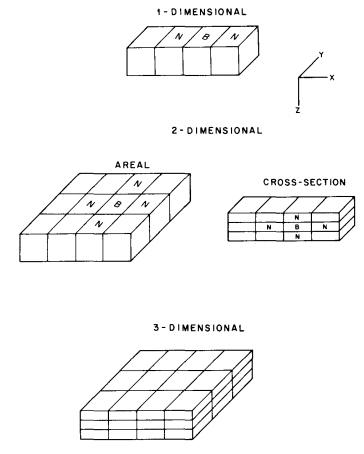
\includegraphics[width=.6\textwidth]{figs/revisao/revisao_DIM}
	\caption{Classifica\c{c}\~{a}o dos simuladores por dimens\~{a}o \cite{coats1982} \label{fig:revisao_DIM}}
\end{figure}

\'{E} importante que, ao se escolher um simulador num\'{e}rico para se resolver problemas de engenharia de reservat\'{o}rio, se considere v\'{a}rios fatores, a saber: o tipo de estudo a ser feito, tipo e caracter\'{i}sticas do reservat\'{o}rio e dos fluidos presentes, quantidade e qualidade dos dados, o detalhamento necess\'{a}rio do estudo e os recursos computacionais dispon\'{i}veis \cite[p. 519]{engres}. Por exemplo, \'{e} impratic\'{a}vel o uso de modelos composicionais em computadores cuja capacidade seja compar\'{a}vel a um computador pessoal de alto desempenho, devido \`{a} complexidade dos c\'{a}lculos envolvidos. Por outro lado, por sua simplicidade, um modelo \textit{black oil} poderia ser considerado, respeitando-se ao m\'{a}ximo as caracter\'{i}sticas do reservat\'{o}rio estudado.

\subsection{Uso de Simuladores Num\'{e}ricos para Estudos de Reservat\'{o}rios}

O uso de simuladores num\'{e}ricos torna poss\'{i}vel analisar o comportamento de um reservat\'{o}rio ao longo do tempo, dado um esquema de produ\c{c}\~{a}o. Dessa forma, pode-se obter, por exemplo, as condi\c{c}\~{o}es \'{o}timas de produ\c{c}\~{a}o, al\'{e}m de se determinar como a inje\c{c}\~{a}o de diferentes tipos de fluidos ou outros m\'{e}todos de EOR afetam o sistema simulado, determinar o efeito da localiza\c{c}\~{a}o dos po\c{c}os na recupera\c{c}\~{a}o de \'{o}leo e/ou g\'{a}s e analisar a influ\^{e}ncia de diferentes vaz\~{o}es de produ\c{c}\~{a}o e/ou inje\c{c}\~{a}o. O simulador obt\'{e}m seus resultados de informa\c{c}\~{o}es de natureza geol\'{o}gica, propriedades da rocha e dos fluidos presentes no meio poroso, hist\'{o}ricos de produ\c{c}\~{a}o (vaz\~{o}es e/ou produ\c{c}\~{o}es acumuladas de \'{o}leo e \'{a}gua) e de press\~{a}o, e outras informa\c{c}\~{o}es a respeito dos po\c{c}os de petr\'{o}leo, assim como as caracter\'{i}sticas de completa\c{c}\~{a}o \cite[pp. 522--523]{engres}. A Figura \ref{fig:revisao_simsec1} ilustra a aplica\c{c}\~{a}o de simuladores num\'{e}ricos para engenharia de reservat\'{o}rios.

\begin{figure}[!ht]
	\centering
	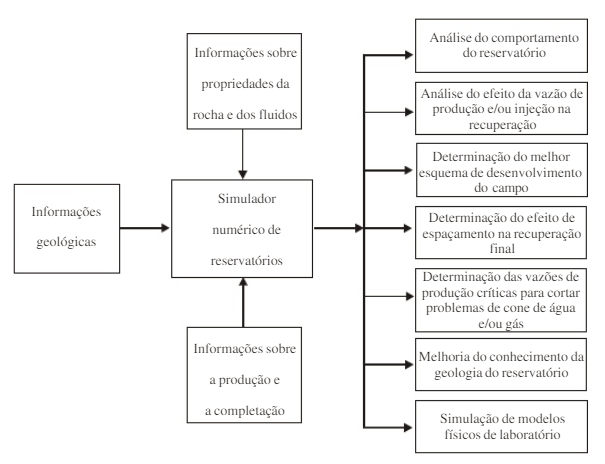
\includegraphics[width=.75\textwidth]{figs/revisao/revisao_simsec1}
	\caption{Aplica\c{c}\~{a}o de simuladores num\'{e}ricos em reservat\'{o}rios \cite[p. 522]{engres}}
	\label{fig:revisao_simsec1}
\end{figure}  

As etapas normalmente seguidas durante a simula\c{c}\~{a}o num\'{e}rica de um reservat\'{o}rio s\~{a}o \footnote{Ver \cite[pp. 523--524]{engres}. Ver tamb\'{e}m \cite{fanchi} para maiores detalhes sobre cada etapa.}:

\begin{enumerate}
\item \textbf{Coleta e prepara\c{c}\~{a}o dos dados:} \'{e} a fase de armazenamento e interpreta\c{c}\~{a}o de todos os dados cab\'{i}veis ao problema, sejam eles geol\'{o}gicos, propriedades da rocha e dos fluidos, entre outros. Quanto maiores a quantidade e a qualidade desses dados, mais confi\'{a}vel ser\'{a} a simula\c{c}\~{a}o. Breitenbach destaca que dados adicionais podem ser necess\'{a}rios considerando-se a dificuldade do problema de mec\^{a}nica dos fluidos e os objetivos de estudo, dependentes de qual processo do reservat\'{o}rio est\'{a} sendo modelado \cite{breitenbach1991}.
\item \textbf{Prepara\c{c}\~{a}o do modelo num\'{e}rico:} Ocorre logo ap\'{o}s a tomada dos dados. Inicialmente, \'{e} feito o \textit{lan\c{c}amento do} grid \textit{ou malha}, onde \'{e} constru\'{i}da uma malha para se transpor as informa\c{c}\~{o}es necess\'{a}rias para o modelo. Logo, \'{e} feita a divis\~{a}o do reservat\'{o}rio em v\'{a}rias c\'{e}lulas, cada uma funcionando como um reservat\'{o}rio menor, conforme mostra a Figura \ref{fig:revisao_simsec3}. Breitenbach ressalta que combina\c{c}\~{o}es de modelos muitas vezes s\~{a}o selecionadas para se estudar, por exemplo, posicionamento de po\c{c}os, fen\^{o}menos de cone, inje\c{c}\~{a}o de fluidos, vaz\~{o}es de produ\c{c}\~{a}o, etc., e que o engenheiro deve utilizar a dimens\~{a}o da malha e os modelos corretos para resolver o problema desejado com as restri\c{c}\~{o}es de custo, tempo e acur\'{a}cia consideradas \cite{breitenbach1991}.
\begin{figure}[H]
	\centering
	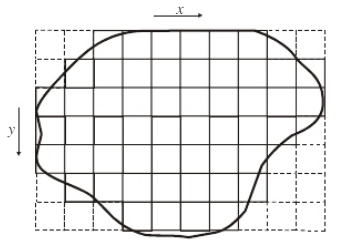
\includegraphics[width=.5\textwidth]{figs/revisao/revisao_simsec3}
	\caption{Malha utilizada na simula\c{c}\~{a}o num\'{e}rica de um reservat\'{o}rio \cite[p. 524]{engres}}
	\label{fig:revisao_simsec3}
\end{figure}
\item \textbf{Ajuste de hist\'{o}rico:} O objetivo desta etapa \'{e} calibrar o modelo num\'{e}rico com o reservat\'{o}rio real a partir dos melhores dados dispon\'{i}veis referentes aos hist\'{o}ricos de produ\c{c}\~{a}o e de press\~{a}o. Oliver e Chen afirmam que se trata de um problema inverso: ao inv\'{e}s de se obter um modelo de reservat\'{o}rio para predizer seu comportamento, a modelagem \'{e} feita a partir da observa\c{c}\~{a}o dos processos ocorridos no reservat\'{o}rio \cite{Oliver2011}\footnote{Oliver e Chen apresentam uma revis\~{a}o da literatura a respeito do ajuste de hist\'{o}rico; ver \cite{Oliver2011}}. O ajuste de hist\'{o}rico \'{e} um c\'{a}lculo do comportamento passado do reservat\'{o}rio e a consequente compara\c{c}\~{a}o com o hist\'{o}rico do campo ou do mesmo reservat\'{o}rio; se a concord\^{a}ncia n\~{a}o \'{e} satisfat\'{o}ria, s\~{a}o necess\'{a}rios ajustes nos dados at\'{e} se obter resultados adequados. De todo modo, a import\^{a}ncia de se obter um bom ajuste de hist\'{o}rico reside no fato de que o modelo poder\'{a} ser utilizado para se efetuar previs\~{o}es confi\'{a}veis em rela\c{c}\~{a}o ao seu comportamento futuro.
\item \textbf{Extrapola\c{c}\~{a}o:} Uma vez que o ajuste de hist\'{o}rico \'{e} realizado, procede-se \`{a} fase de extrapola\c{c}\~{a}o, isto \'{e}, a previs\~{a}o de comportamento futuro do modelo. Podem ser impostas vaz\~{o}es e press\~{o}es para todos os po\c{c}os, condi\c{c}\~{o}es dessas vaz\~{o}es, entre outros. Essa etapa permite avaliar v\'{a}rios esquemas de produ\c{c}\~{a}o, e seus resultados podem ser utilizados em avalia\c{c}\~{o}es econ\^{o}micas, tornando poss\'{i}vel decidir pelo esquema \'{o}timo de produ\c{c}\~{a}o, conforme tamb\'{e}m sugere Fanchi \footnote{Ver \cite[p. 373]{fanchi}.}.
\end{enumerate}

Todas as etapas de simula\c{c}\~{a}o num\'{e}rica de reservat\'{o}rios est\~{a}o resumidos na Figura \ref{fig:revisao_simsec2}.

\begin{figure}[!ht]
	\centering
	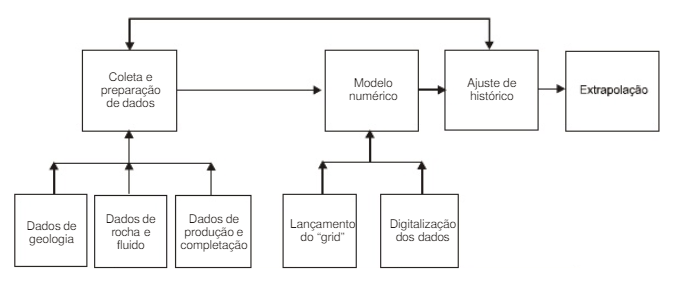
\includegraphics[width=.75\textwidth]{figs/revisao/revisao_simsec2}
	\caption{Etapas da simula\c{c}\~{a}o num\'{e}rica de um reservat\'{o}rio \cite[p. 523]{engres}}
	\label{fig:revisao_simsec2}
\end{figure}
%TCIDATA{LaTeXparent=0,0,cap_RevisaoBibliografica.tex}

\section{Conceitos de Otimiza\c{c}\~{a}o}\label{subsec:otimconcepts}

\subsection{Defini\c{c}\~{o}es e Fatos B\'{a}sicos}
Antes de se proceder \`{a} an\'{a}lise do problema estudado, fazem-se necess\'{a}rios alguns conceitos b\'{a}sicos da \'{a}rea de otimiza\c{c}\~{a}o e \'{a}lgebra linear. A presente se\c{c}\~{a}o apresenta algumas defini\c{c}\~{o}es que ser\~{a}o importantes ao descorrer da an\'{a}lise de convexidade e de problemas de otimiza\c{c}\~{a}o. Primeiramente, s\~{a}o dadas algumas defini\c{c}\~{o}es sobre vetores e matrizes, conforme Aguirre \cite{aguirre}:
\begin{definition}\label{dotProd}
Dadas duas vari\'{a}veis $\mathbf{x} \in \mathbb{R}^{n}$ e $\mathbf{y} \in \mathbb{R}^{n}$, o \textit{produto interno} entre $\mathbf{x}$ e $\mathbf{y}$ \'{e} dado por $\left\langle \mathbf{x},\mathbf{y}\right\rangle = \mathbf{x}^{T}\mathbf{y} = \mathbf{y}^{T}\mathbf{x}$. Caso este produto seja nulo, os vetores s\~{a}o ditos \textit{ortogonais}.
\end{definition}
\begin{definition}
Uma matriz $\mathbf{A} \in \mathbb{R}^{n \times n}$ \'{e} dita \textit{semidefinida positiva} se $\mathbf{x}^{T}\mathbf{A}\mathbf{x} \ge \mathbf{0}, \forall\mathbf{x} \ne \mathbf{0}, \mathbf{x} \in \mathbb{R}^{n}$. No caso de desigualdade estrita, a matriz $\mathbf{A}$ \'{e} dita \textit{definida positiva}. 
\end{definition}

\begin{definition}
Uma matriz $\mathbf{A} \in \mathbb{R}^{n \times n}$ \'{e} dita \textit{semidefinida negativa} se $\mathbf{x}^{T}\mathbf{A}\mathbf{x} \le \mathbf{0}, \forall\mathbf{x} \ne \mathbf{0}, \mathbf{x} \in \mathbb{R}^{n}$. No caso de desigualdade estrita, a matriz $\mathbf{A}$ \'{e} dita \textit{definida negativa}. 
\end{definition}

\begin{definition}
Uma matriz $\mathbf{A} \in \mathbb{R}^{n \times n}$ \'{e} dita \textit{indefinida} se ela n\~{a}o for semidefinida positiva nem semidefinida negativa.
\end{definition}

Uma \'{u}ltima defini\c{c}\~{a}o b\'{a}sica de \'{a}lgebra linear se refere ao conceito de normas de vetores e matrizes, de acordo com Yang \cite{yang}:

\begin{definition} \label{pNorm}
Seja $\mathbf{v} \in \mathbb{R}^{n}$. A \textit{p-norma} ou $\ell_p$\textit{-norma} de $v$ \'{e} dada por
\begin{equation}
	\label{vecNorm}
	\left\|\mathbf{v}\right\|_{p} = \left(\sum_{i=1}^{n}\lvert v_i \rvert ^{p}\right)^{\frac{1}{p}},~p \in \mathbb{Z}_{+} - \left\lbrace 0\right\rbrace.
\end{equation}
\end{definition}
Algumas propriedades elementares da norma vetorial devem ser satisfeitas para todo valor de $p$, entre as quais:
\begin{enumerate}[label=(\alph*)]
\item $\left\|\mathbf{v}\right\| \ge 0 ,~ \forall \mathbf{v}$;
\item $\left\|\mathbf{v}\right\| = 0 \Rightarrow \mathbf{v} = \mathbf{0}$;
\item $\left\|\alpha\mathbf{v}\right\| = \lvert\alpha\rvert \left\|\mathbf{v}\right\|,~ \forall \alpha \in \mathbb{R}$;
\item $\left\|\mathbf{u} + \mathbf{v}\right\| \le \left\|\mathbf{u}\right\| + \left\|\mathbf{v}\right\|$ (Desigualdade triangular).
\end{enumerate}

Algumas normas vetoriais comuns s\~{a}o calculadas tomando-se \eqref{vecNorm} com $p = 1$ e $p = 2$, sendo a \textit{2-norma} de $\mathbf{v}$ tamb\'{e}m conhecida como \textit{norma euclidiana}, ou \textit{comprimento} de $\mathbf{v}$. Neste caso, a norma de $v$ tamb\'{e}m pode ser escrita como
\begin{equation}
	\left\|\mathbf{v}\right\|_{2} = \sqrt{\mathbf{v}^T\mathbf{v}}.
\end{equation} 

Um caso especial de norma vetorial ocorre quando $p = \infty$; a $\ell_{\infty}$-norma, ou \textit{norma de Chebyshev} de $\mathbf{v}$, \'{e} dada por
\begin{equation}
\left\|\mathbf{v}\right\|_{p} = v_{max} = \max_{1 \le i \le n} \lvert v_i \rvert.
\end{equation}

\begin{definition}
Dada uma matriz $\mathbf{A} \in \mathbb{R}^{m \times n}$ qualquer, a sua \textit{$p$-norma}, analogamente \`{a} Defini\c{c}\~{a}o \ref{pNorm}, pode ser escrita como
\begin{equation}
	\label{matNorm}
	\left\|\mathbf{A}\right\|_{p} = \left(\sum_{i=1}^{m} \sum_{j=1}^{n}\lvert a_{ij} \rvert ^{p}\right)^{\frac{1}{p}},~p \in \mathbb{Z}_{+} - \left\lbrace 0\right\rbrace.
\end{equation}
\end{definition} 

Um caso especial da norma matricial ocorre quando se aplica a Equa\c{c}\~{a}o \eqref{matNorm} com $p = 2$; tal norma \'{e} denominada \textit{norma de Frobenius} de $\mathbf{A}$. Outras normas matriciais populares s\~{a}o tidas como a m\'{a}xima soma de linhas ou de colunas da matriz ($\left\|\mathbf{A}\right\|_{1}$ e $\left\|\mathbf{A}\right\|_{\infty}$, respectivamente). Deve-se destacar tamb\'{e}m que todas as propriedades b\'{a}sicas satisfeitas para a norma vetorial devem ser verdadeiras tamb\'{e}m para a norma matricial.

Outros conceitos b\'{a}sicos a serem apresentados s\~{a}o pertencentes \`{a} \'{a}rea de otimiza\c{c}\~{a}o. Izmailov e Solodov \cite{izmailov} trazem o conceito elementar de problema de otimiza\c{c}\~{a}o e m\'{i}nimo (ou m\'{a}ximo) de uma fun\c{c}\~{a}o:

\begin{definition} 
Sejam um conjunto $D \subset \mathbb{R}^{n}$ e uma fun\c{c}\~{a}o $f: D \to \mathbb{R}$. O problema de se encontrar uma minimizador de $f$ em $D$ \'{e} escrito como
\begin{equation}
\label{basicProb}
\min f(\mathbf{x}) \text{ sujeito a } \mathbf{x} \in D.
\end{equation} A fun\c{c}\~{a}o $f$ \'{e} denominada \textit{fun\c{c}\~{a}o objetivo}; o conjunto $D$ \'{e} o \textit{conjunto vi\'{a}vel} do problema, ou \textit{conjunto de restri\c{c}\~{o}es} --- seus pontos ser\~{a}o chamados de \textit{pontos vi\'{a}veis}. Normalmente, o conjunto de restri\c{c}\~{o}es $D$ pode ser definido como
\begin{equation}
D = \left\lbrace \mathbf{x} \in \Omega \mid h(\mathbf{x}) = 0, g(\mathbf{x}) < 0 \right\rbrace
\end{equation} em que $\Omega$ \'{e} o conjunto de \textit{restri\c{c}\~{o}es diretas} do problema ($\Omega \subset \mathbb{R}^{n}$), $h: \Omega \to \mathbb{R}^{l}$ e $g: \Omega \to \mathbb{R}^{m}$ s\~{a}o as $l \in \mathbb{Z}_{+}$ restri\c{c}\~{o}es de igualdade e $m \in \mathbb{Z}_{+}$ restri\c{c}\~{o}es de desigualdade (tamb\'{e}m denomiadas \textit{restri\c{c}\~{o}es funcionais}). Caso $D = \mathbb{R}^{n}$, o problema \'{e} dito de \textit{otimiza\c{c}\~{a}o irrestrita}; em caso contr\'{a}rio, se trata de problema com restri\c{c}\~{o}es.
\end{definition} 
\begin{definition} 
Um problema de maximiza\c{c}\~{a}o pode ser escrito como
\begin{equation}
\label{def2_4}
\max f(\mathbf{x}) \text{ sujeito a } \mathbf{x} \in D.
\end{equation} 
Nota-se que o problema \eqref{def2_4} pode ser reescrito como um problema de minimiza\c{c}\~{a}o equivalente:
\begin{equation*}
\min -f(\mathbf{x}) \text{ sujeito a } \mathbf{x} \in D.
\end{equation*}
\end{definition}  
Visto que resolver um problema de maximiza\c{c}\~{a}o n\~{a}o exige t\'{e}cnicas substancialmente diferentes de um problema de minimiza\c{c}\~{a}o, uma vez que um pode ser reescrito como o outro, ser\~{a}o considerados a partir dessa se\c{c}\~{a}o problemas de minimiza\c{c}\~{a}o.

Antes de se prosseguir com os conceitos de minimizador e valor \'{o}timo, s\~{a}o necess\'{a}rios os
conceitos de supremo, \'{i}nfimo, m\'{a}ximos e m\'{i}nimos de um conjunto. A defini\c{c}\~{a}o a seguir \'{e} encontrada em Yang \cite{yang}:
\begin{definition} \label{defSupInf}
Dado um conjunto $S \in \mathbb{R}$, o n\'{u}mero $u$ \'{e} denominado \textit{limite superior} de $S$ se $u \ge x, ~ \forall x \in S$. Por consequ\^{e}ncia, o n\'{u}mero $\beta$ \'{e} denominado \textit{supremo} de $S$ se $\beta$ \'{e} o menor dos limites superiores $u$ de $S$ ($\beta \le u ,~\forall u$). O supremo de $S$ pode ser denotado por
\begin{equation}
\beta \equiv \sup_{x \in S} x \equiv \sup S \equiv \sup(S).
\end{equation}
Caso $\beta \in S$, pode-se dizer que $\beta$ \'{e} o \textit{valor m\'{a}ximo} de $S$, ou seja,
\begin{equation}
\beta \equiv \max S \equiv \max(S).
\end{equation}

De maneira an\'{a}loga, o n\'{u}mero $l$ \'{e} denominado \textit{limite inferior} de $S$ se $l \le x, ~ \forall x \in S$. Por consequ\^{e}ncia, o n\'{u}mero $\alpha$ \'{e} denominado \textit{\'{i}nfimo} de $S$ se $\alpha$ \'{e} o maior dos limites inferiores $l$ de $S$ ($\alpha \ge l ,~\forall l$). O \'{i}nfimo de $S$ pode ser denotado por
\begin{equation}
\alpha \equiv \inf_{x \in S} x \equiv \inf S \equiv \inf(S).
\end{equation}
Caso $\alpha \in S$, pode-se dizer que $\alpha$ \'{e} o \textit{valor m\'{i}nimo} de $S$, ou seja,
\begin{equation}
\alpha \equiv \min S \equiv \min(S).
\end{equation}
\end{definition} 

Algumas propriedades b\'{a}sicas sobre \'{i}nfimos e supremos s\~{a}o apresentadas a seguir, de acordo com Yang \cite{yang}:
\begin{equation}
\inf Q = -\sup(-Q),
\end{equation}
\begin{equation}
\sup_{p \in P, q \in Q} (p+q) = sup(P) + sup(Q),
\end{equation}
\begin{equation}
\sup_{x \in S}\left(f(x)+g(x)\right) \le \sup_{x \in S}\left(f(x)\right) + \sup_{x \in S}\left(g(x)\right).
\end{equation}

Vale notar que os conceitos de supremo e \'{i}nfimo apresentados n\~{a}o extendem a conjuntos n\~{a}o-limitados; por exemplo, seja o conjunto $S = \left[ 2,+\infty \right)$. Verifica-se que, de acordo com a Defini\c{c}\~{a}o \ref{defSupInf}, $\inf S = 2$, mas o supremo n\~{a}o existe, ou seja, $\sup S \to +\infty$. Por este exemplo, conclui-se que \'{i}nfimos ou supremos podem n\~{a}o existir em conjuntos n\~{a}o limitados; portanto, para contornar este fato, faz-se a defini\c{c}\~{a}o de uma extens\~{a}o dos n\'{u}meros reais \cite{yang}: 
\begin{equation}
\label{altR}
\bar{\mathbb{R}} = \mathbb{R} \cup \left\lbrace \pm \infty \right\rbrace.
\end{equation}

Considerando-se a Equa\c{c}\~{a}o \eqref{altR} e que $\sup(\emptyset) = -\infty$, para qualquer subconjunto de $\bar{\mathbb{R}}$, o supremo e \'{i}nfimo sempre existir\~{a}o, supondo-se $\sup \mathbb{R} = +\infty$ e $\inf \mathbb{R} = -\infty$.

De posse das defini\c{c}\~{o}es at\'{e} aqui dadas, \'{e} poss\'{i}vel definir os conceitos de minimizador e valor \'{o}timo de uma fun\c{c}\~{a}o. As defini\c{c}\~{o}es a seguir s\~{a}o dadas por Izmailov e Solodov \cite{izmailov}:

\begin{definition} 
Dado o problema \eqref{basicProb}, diz-se que um ponto $\bar{\mathbf{x}} \in D$ \'{e}
\begin{enumerate}[label=(\alph*)]
\item \textit{minimizador global} de \eqref{basicProb}, se
\begin{equation}
\label{globalMin}
f(\bar{\mathbf{x}}) \le f(\mathbf{x}) ~ \forall \mathbf{x} \in D;
\end{equation}
\item \textit{minimizador local} de \eqref{basicProb}, se existe uma vizinhan\c{c}a $U$ de $\bar{\mathbf{x}}$ tal que
\begin{equation}
\label{localMin}
f(\bar{\mathbf{x}}) \le f(\mathbf{x}) ~ \forall \mathbf{x} \in D \cap U,
\end{equation} ou, de forma an\'{a}loga,
\begin{equation}
\exists \epsilon > 0 ~ \bullet ~ f(\bar{\mathbf{x}}) \le f(\mathbf{x}) ~ \forall \mathbf{x} \in \left\lbrace \mathbf{x} \in D \mid \left\|\mathbf{x} - \bar{\mathbf{x}} \right\| \le \epsilon \right\rbrace.
\end{equation}
\end{enumerate}
\end{definition} 

Observa-se que todo minimizador global \'{e} tamb\'{e}m local, mas n\~{a}o de forma rec\'{i}proca. Se, para $\mathbf{x} \ne \bar{\mathbf{x}}$, a desigualdade \eqref{globalMin} ou \eqref{localMin} \'{e} estrita, $\bar{\mathbf{x}}$ \'{e} chamado de \textit{minimizador estrito} (global ou local, respectivamente).

\begin{definition} 
Seja $\bar{\mathbf{v}} \in \left[ -\infty,+\infty \right)$ definido por
\begin{equation}
\bar{\mathbf{v}} = \inf_{\mathbf{x} \in D} f(\mathbf{x});
\end{equation}
neste caso, $\bar{\mathbf{v}}$ \'{e} denominado \textit{valor \'{o}timo} do problema \eqref{basicProb}.
\end{definition} 

\subsection{Diferenciabilidade de Fun\c{c}\~{o}es Multivari\'{a}veis e Campos Vetoriais}

Antes de se proceder \`{a} an\'{a}lise de fun\c{c}\~{o}es que possuem dom\'{i}nio ou contradom\'{i}nio (ou ambos) multidimensionais, ser\'{a} feita uma diferencia\c{c}\~{a}o conceitual entre fun\c{c}\~{o}es multivari\'{a}veis e campos vetoriais (fun\c{c}\~{o}es multiobjetivo):

\begin{definition}
Uma aplica\c{c}\~{a}o $f(\mathbf{x}): A \to B,~ A \subset \mathbb{R}^{n}$ \'{e} denominada fun\c{c}\~{a}o multivari\'{a}vel se seu contradom\'{i}nio \'{e} subconjunto dos n\'{u}meros reais, isto \'{e}, $B \subset \mathbb{R}$.
\end{definition}

\begin{definition}
Uma aplica\c{c}\~{a}o $\mathbf{F}(\mathbf{x}): A \to B,~ A \subset \mathbb{R}^{n}$ \'{e} denominada campo vetorial (ou fun\c{c}\~{a}o multiobjetivo) se seu contradom\'{i}nio \'{e} subconjunto de um espa\c{c}o euclidiano de dimens\~{a}o $m > 1$, isto \'{e}, $B \subset \mathbb{R}^{m}$.
\end{definition}

O conceito de continuidade, nesses casos, pode ser visto como uma extens\~{a}o da Defini\c{c}\~{a}o \ref{scalarCont}\footnote{Ver \cite[p. 301]{thomas2}.}; por\'{e}m, o conceito de diferenciabilidade deve ser largamente extendido, pois agora, ao contr\'{a}rio do caso escalar, o n\'{u}mero de dire\c{c}\~{o}es poss\'{i}veis \'{e} infinito. Em casos em que essas dire\c{c}\~{o}es correspondem aos vetores da base can\^{o}nica do espa\c{c}o do dom\'{i}nio ($\mathbf{e_i} = (0,...,1,...,0)$ com o elemento n\~{a}o-nulo na $i$-\'{e}sima posi\c{c}\~{a}o), as derivadas de uma fun\c{c}\~{a}o vetorial nessas dire\c{c}\~{o}es s\~{a}o conhecidas como \textit{derivadas parciais}.

\begin{definition}\footnote{Adaptado de \cite[p. 308]{thomas2}.}
Dizemos que a \textit{derivada parcial} de $f(\mathbf{x})$ em rela\c{c}\~{a}o \`{a} componente $x_i$ \'{e} equivalente ao limite
\begin{equation}
\frac{\partial}{\partial x_i}f(\mathbf{x}) \equiv \frac{\partial f}{\partial x} \equiv f_{x_i}(\mathbf{x}) = \lim_{h \to 0} \frac{f(x_1,...,x_i + h,...,x_n)-f(\mathbf{x})}{h},
\end{equation}
desde que tal limite exista.
\end{definition}

Quando todas as derivadas parciais de uma fun\c{c}\~{a}o $f(\mathbf{x})$ existem, o \textit{gradiente} de $f$ \'{e} dado, por defini\c{c}\~{a}o, como
\begin{equation}
\nabla f := (\frac{\partial f}{\partial x_1},\frac{\partial f}{\partial x_2},...,\frac{\partial f}{\partial x_n})
\end{equation}

A principal diferen\c{c}a entre fun\c{c}\~{o}es com dom\'{i}nio multidimensional e as escalares reside no fato de que o n\'{u}mero de dire\c{c}\~{o}es poss\'{i}veis n\~{a}o \'{e} finito; como as derivadas parciais apenas consideram as dire\c{c}\~{o}es da base do espa\c{c}o, um novo conceito de derivada \'{e} necess\'{a}rio. Para tanto, seja o vetor $\mathbf{d} \in \mathbb{R}^{n}$ definido como
\begin{equation*}
\mathbf{d} = (d_1,d_2,...,d_n) = \sum_{i=1}^{n} d_i\mathbf{e_i}
\end{equation*}
com $\mathbf{e_i}$ sendo o $i$-\'{e}simo vetor de coordenadas, conceito j\'{a} discutido anteriormente. Esse vetor $\mathbf{d}$ pode ser entendido como uma \textit{dire\c{c}\~{a}o} em $\mathbb{R}^{n}$. A defini\c{c}\~{a}o a seguir de derivada direcional se encontra em Guller \cite{guller}:
 
\begin{definition}\label{direcDif}
A derivada direcional de $f$ em um ponto $\mathbf{x}$ de seu dom\'{i}nio na dire\c{c}\~{a}o $\mathbf{d} \in \mathbb{R}^{n}$ \'{e} dada por
\begin{equation}
f'(\mathbf{x};\mathbf{d}) = \lim_{t \searrow 0} \frac{f(\mathbf{x}+t\mathbf{d})-f(\mathbf{x})}{t},
\end{equation}
desde que o limite exista \`{a} medida que $t \ge 0$ se aproxima de $0$.
\end{definition}

Guller ainda destaca que, al\'{e}m do fato de que $f'(\mathbf{x};\alpha\mathbf{d}) = \alpha f'(\mathbf{x};\mathbf{d})$ para $\alpha \ge 0$, a derivada direcional pode ser calculada como mostrado a seguir, se $f'(\mathbf{x};-\mathbf{d}) = -f'(\mathbf{x};\mathbf{d})$:
\begin{equation*}
f'(\mathbf{x};\mathbf{d}) = \lim_{t \to 0} \frac{f(\mathbf{x}+t\mathbf{d})-f(\mathbf{x})}{t}.
\end{equation*}

Fica claro que, quando a dire\c{c}\~{a}o $\mathbf{d}$ equivale a algum vetor de coordenadas de $\mathbb{R}^{n}$, como $\mathbf{e_i}$, aplicar a Defini\c{c}\~{a}o \ref{direcDif} implica em calcular a derivada parcial de $f$ na coordenada $x_i$, ou seja,
\begin{equation*}
f'(\mathbf{x};\mathbf{e_i}) \equiv \frac{\partial f}{\partial x_i}.
\end{equation*}
Com isso, permite-se concluir que a no\c{c}\~{a}o de derivada direcional \'{e} uma generaliza\c{c}\~{a}o da derivada parcial para qualquer dire\c{c}\~{a}o.

Antes de se prosseguir com a an\'{a}lise de diferencia\c{c}\~{a}o de fun\c{c}\~{o}es multivari\'{a}veis e campos vetoriais, faz-se necess\'{a}rio apresentar uma nota\c{c}\~{a}o que ser\'{a} utilizada posteriormente, a \textit{nota\c{c}\~{a}o de Landau (``o'' pequeno)}:

\begin{definition}[Nota\c{c}\~{a}o de Landau]\footnote{Ver \cite[p. 6]{guller}}
Segundo a nota\c{c}\~{a}o de Landau, um vetor pode ser chamado $o(\mathbf{h}) \in \mathbb{R}^{n}$ se
\begin{equation*}
\lim_{\mathbf{h} \to \mathbf{0}} \frac{\norm{o(\mathbf{h})}}{\norm{\mathbf{h}}} = 0.
\end{equation*}
\end{definition}

\begin{definition}\label{gateauxDef}\footnote{\textit{Ibid., p. 6.}}
Uma fun\c{c}\~{a}o $f: U \subseteq \mathbb{R}^{n} \to \mathbb{R}$ \'{e} dita \textit{G\^{a}teaux diferenci\'{a}vel} em $\mathbf{x} \in U$ se a derivada direcional $f'(\mathbf{x};\mathbf{d})$ existe para toda dire\c{c}\~{a}o $\mathbf{d} \in \mathbb{R}^{n}$ e \'{e} uma fun\c{c}\~{a}o linear de $\mathbf{d}$.
\end{definition}

Pela defin\c{c}\~{a}o de diferenciabilidade de G\^{a}teaux e utilizando a defini\c{c}\~{a}o de dire\c{c}\~{a}o, a derivada de G\^{a}teaux pode ser calculada como
\begin{equation}\label{gateauxCalc}
f'(\mathbf{x};\mathbf{d}) = f'(\mathbf{x};\sum_{i=1}^{n}d_i\mathbf{e_i}) = \sum_{i=1}^{n} d_i f'(\mathbf{x};\mathbf{e_i}) = \sum_{i = 1}^{n} d_i \frac{\partial f}{\partial x_i} = \left\langle \mathbf{d},\nabla f \right\rangle = \mathbf{d}^T \nabla f.
\end{equation}

\begin{definition}\label{frechetDef}\footnote{\textit{Ibid., p.6}}
Uma fun\c{c}\~{a}o $f: U \subseteq \mathbb{R}^{n} \to \mathbb{R}$ \'{e} dita \textit{Fr\'{e}chet diferenci\'{a}vel} em $\mathbf{x} \in U$ se existe uma fun\c{c}\~{a}o linear $\ell: \mathbb{R}^{n} \to \mathbb{R},~\ell(\mathbf{x}) = \mathbf{l}^T\mathbf{x}$, tal que
\begin{equation*}
\lim_{\norm{\mathbf{h}} \to 0} \frac{f(\mathbf{x} + \mathbf{h}) - f(\mathbf{x}) - \mathbf{l}^T\mathbf{h}}{\norm{\mathbf{h}}} = 0.
\end{equation*}
\end{definition}

Dizer que uma fun\c{c}\~{a}o $f$ \'{e} Fr\'{e}chet diferenci\'{a}vel em $\mathbf{x}$ equivale a dizer que
\begin{equation}
\label{frechetEqu}
f(\mathbf{x} + \mathbf{h}) = f(\mathbf{x}) + \mathbf{l}^T\mathbf{h} + o(\mathbf{h})
\end{equation}

Dois fatos importantes podem ser retirados da Equa\c{c}\~{a}o \eqref{frechetEqu}; o primeiro \'{e} que, se tomarmos o limite quando $\mathbf{h} \to \mathbf{0}$, tem-se que $\lim_{\mathbf{h} \to \mathbf{0}} f(\mathbf{x} + \mathbf{h}) = f(\mathbf{x})$; isto equivale a dizer que, se $f$ \'{e} Fr\'{e}chet diferenci\'{a}vel em $\mathbf{x}$, ela \'{e} cont\'{i}nua nesse ponto. O outro fato a ser analisado pressup\~{o}e que $\mathbf{l}$ pode ser escolhido como $\nabla f$; neste caso, aplicando-se tamb\'{e}m a Defini\c{c}\~{a}o \ref{dotProd}, \eqref{frechetEqu} se torna
\begin{equation}
\label{frechetEqu2}
f(\mathbf{x} + \mathbf{h}) = f(\mathbf{x}) + \mathbf{h}^T \nabla f + o(\mathbf{h}).
\end{equation}

Claramente, de acordo com a Equa\c{c}\~{a}o \ref{gateauxCalc}, o segundo termo \'{e} a derivada de G\^{a}teaux de $f$ em $\mathbf{x}$ na dire\c{c}\~{a}o $\mathbf{h}$. Portanto, $f$ Fr\'{e}chet diferenci\'{a}vel em $\mathbf{x}$ implica em $f$ G\^{a}teaux diferenci\'{a}vel em $\mathbf{x}$.

A segunda derivada de uma fun\c{c}\~{a}o multivari\'{a}vel requer aten\c{c}\~{a}o especial: uma vez que a primeira derivada, ou gradiente, \'{e} um vetor, a segunda derivada de uma fun\c{c}\~{a}o $f: U \subseteq \mathbb{R}^{n} \to \mathbb{R}$ \'{e} uma matriz quadrada de ordem $n$. Essa matriz \'{e} conhecida como \textit{Hessiana}.

\begin{definition}\footnote{Adaptado de \cite[p. 51]{yang}.}
A segunda derivada de uma fun\c{c}\~{a}o $f: U \subseteq \mathbb{R}^{n} \to \mathbb{R}$, tamb\'{e}m conhecida como Hessiana de $f$, \'{e} dada por
\begin{equation}
H(f) \equiv \nabla^2 f \equiv f''(\mathbf{x}) = [h_{ij}],~h_{ij} = \frac{\partial^2 f}{\partial x_i \partial x_j}.
\end{equation}
\end{definition}

Um fato interessante sobre a Hessiana \'{e} que, se as segundas derivadas parciais de $f$ existem e s\~{a}o cont\'{i}nuas, tem-se que $\frac{\partial^2 f}{\partial x_i \partial x_j} = \frac{\partial^2 f}{\partial x_j \partial x_i}$; neste caso, temos que $H(f) = H^{T}(f)$, ou seja, tem-se $H(f)$ sim\'{e}trica. Este fato \'{e} largamente utilizado em alguns algoritmos de otimiza\c{c}\~{a}o, particularmente em problemas de programa\c{c}\~{a}o quadr\'{a}tica.

Todos os conceitos vistos at\'{e} aqui para fun\c{c}\~{o}es $f: \mathbb{R}^{n} \to \mathbb{R}$ podem ser tamb\'{e}m aplicados a campos vetoriais $\mathbf{F}: \mathbb{R}^{n} \to \mathbb{R}^{m}$. Os conceitos de diferenciabilidade segundo G\^{a}teaux e Fr\'{e}chet s\~{a}o an\'{a}logos aos presentes nas Defini\c{c}\~{o}es \ref{gateauxDef} e \ref{frechetDef} \footnote{Ver \cite[pp. 8-9]{guller}.}. Guller ainda afirma que, se um campo $\mathbf{F}(\mathbf{x})$ \'{e} G\^{a}teaux (ou Fr\'{e}chet) diferenci\'{a}vel em $\mathbf{x}$, ent\~{a}o suas fun\c{c}\~{o}es componentes $f_i(\mathbf{x})$ s\~{a}o G\^{a}teaux (ou Fr\'{e}chet) diferenci\'{a}veis em $\mathbf{x}$. A mudan\c{c}a aqui \'{e} o c\'{a}lculo da derivada de $\mathbf{F}$, agora uma matriz.

\begin{definition}\footnote{Adaptado de \cite[p. 9]{guller}.}
Dado um campo vetorial $\mathbf{F}: \mathbb{R}^{n} \to \mathbb{R}^{m}$, sua derivada, denominada Jacobiana de $\mathbf{F}$, \'{e} dada por
\begin{equation}
J(\mathbf{F}) = \left[ \frac{\partial f_i}{\partial x_j} \right].
\end{equation}
\end{definition}

Nota-se, pela defini\c{c}\~{a}o de Jacobiana, que o conceito de gradiente de uma fun\c{c}\~{a}o multivari\'{a}vel \'{e} um caso espec\'{i}fico de Jacobiana, assim como uma fun\c{c}\~{a}o multivari\'{a}vel \'{e} um tipo especial de campo vetorial, em que o contradom\'{i}nio \'{e} unidimensional.

\subsection{Convexidade}
Segundo Izmailov e Solodov \cite{izmailov}, o conceito de convexidade \'{e} muito importante na teoria de otimiza\c{c}\~{a}o; com no\c{c}\~{o}es de convexidade, condi\c{c}\~{o}es de otimalidade necess\'{a}rias passam a ser suficientes, ou seja, basta encontrar um ponto estacion\'{a}rio para o problema. Em particular, sob condi\c{c}\~{o}es de convexidade, todo minimizador local torna-se global. Outra possibilidade poss\'{i}vel utilizando convexidade \'{e} o uso da teoria da dualidade na sua forma mais completa, ou seja, \'{e} poss\'{i}vel associar o problema original (primal) a um problema alternativo (dual) que \'{e}, em determinadas condi\c{c}\~{o}es, equivalente ao original e \`{a}s vezes de mais f\'{a}cil resolu\c{c}\~{a}o. Por fim, o conceito de convexidade possibilita o uso de uma das condi\c{c}\~{o}es de otimalidade mais poderosas aplicadas a problemas com restri\c{c}\~{o}es: as condi\c{c}\~{o}es KKT.

\begin{definition}
Um conjunto $D \subset \eucR{n}$ \'{e} dito convexo se, para quaisquer $\mathbf{x} \in D,~\mathbf{y} \in D$ e $\alpha \in [0,1]$, tem-se $\alpha\mathbf{x} + (1-\alpha)\mathbf{y} \in D$.
\end{definition}

O ponto $\alpha\mathbf{x} + (1-\alpha)\mathbf{y},~\alpha \in [0,1]$, \'{e} conhecido como a \textit{combina\c{c}\~{a}o convexa} de $\mathbf{x}$ e $\mathbf{y}$, com par\^{a}metro $\alpha$.

Em termos de convexidade de uma fun\c{c}\~{a}o, as defini\c{c}\~{o}es a seguir s\~{a}o adaptadas de Izmailov e Solodov\footnote{Ver \cite[pp. 66-70]{izmailov}.}. Sup\~{o}e-se, para todas as defini\c{c}\~{o}es, que o conjunto $D \subset \eucR{n}$ presente nelas \'{e} convexo.

\begin{definition}\label{convDef}
Uma fun\c{c}\~{a}o $f: D \to \setR$ \'{e} convexa em $D$ se, para quaisquer $\mathbf{x} \in D,~\mathbf{y} \in D$ e $\alpha \in [0,1]$, tem-se
\begin{equation}
f(\alpha\mathbf{x} + (1-\alpha)\mathbf{y}) \le \alpha f(\mathbf{x}) + (1-\alpha)f(\mathbf{y}).
\end{equation}
\end{definition}

\begin{definition}
Uma fun\c{c}\~{a}o $f: D \to \setR$ \'{e} estritamente convexa em $D$ se, para quaisquer $\mathbf{x} \in D,~\mathbf{y} \in D, \mathbf{x} \ne \mathbf{y}$ e $\alpha \in (0,1)$, tem-se
\begin{equation}
f(\alpha\mathbf{x} + (1-\alpha)\mathbf{y}) < \alpha f(\mathbf{x}) + (1-\alpha)f(\mathbf{y}).
\end{equation}
\end{definition}

\begin{definition}
Uma fun\c{c}\~{a}o $f: D \to \setR$ \'{e} fortemente convexa em $D$, com m\'{o}dulo $\gamma > 0$ se, para quaisquer $\mathbf{x} \in D,~\mathbf{y} \in D$ e $\alpha \in [0,1]$, tem-se
\begin{equation}
f(\alpha\mathbf{x} + (1-\alpha)\mathbf{y}) \le \alpha f(\mathbf{x}) + (1-\alpha)f(\mathbf{y}) - \gamma\alpha(1-\alpha)\norm{\mathbf{x}-\mathbf{y}}^2.
\end{equation}
\end{definition}

Vale notar que uma fun\c{c}\~{a}o fortemente convexa \'{e} estritamente convexa, e que uma fun\c{c}\~{a}o estritamente convexa \'{e} uma fun\c{c}\~{a}o convexa; a rec\'{i}proca, por\'{e}m, nem sempre \'{e} verdadeira.

\begin{definition}
Uma fun\c{c}\~{a}o $f: D \to \setR$ \'{e} c\^{o}ncava em $D$ se $-f$ for convexa em $D$.
\end{definition}

\begin{definition}\label{concaveDef}
O problema de otimiza\c{c}\~{a}o \eqref{basicProb} \'{e} um problema de minimiza\c{c}\~{a}o convexo quando $D$ \'{e} um conjunto convexo e $f$ \'{e} uma fun\c{c}\~{a}o convexa.
\end{definition}

Uma vez que a fun\c{c}\~{a}o e o conjunto de restri\c{c}\~{o}es s\~{a}o convexos, resolver um problema de otimiza\c{c}\~{a}o torna-se menos tortuoso; encontrar um minimizador \'{e} garantido. A import\^{a}ncia desse fato pode ser vista no teorema a seguir, retirado de Izmailov e Solodov \footnote{Ver \cite[p. 69]{izmailov}. Ver prova em \cite[pp. 69-70]{izmailov}.}.

\begin{theorem}[Teorema de minimiza\c{c}\~{a}o convexa]\label{theoMinConv}
Todo minimizador local de um problema convexo \'{e} um minimizador global, e o conjunto de minimizadores \'{e} convexo. Al\'{e}m disso, se a fun\c{c}\~{a}o objetivo for estritamente convexa, s\'{o} h\'{a} no m\'{a}ximo um minimizador.
\end{theorem}

Uma vez que resolver um problema de maximiza\c{c}\~{a}o \'{e} an\'{a}logo a resolver um problema de minimiza\c{c}\~{a}o, o teorema acima pode ser adaptado com o conceito de concavidade visto na Defini\c{c}\~{a}o \ref{concaveDef}: o problema a ser resolvido neste caso se trata de maximiza\c{c}\~{a}o de uma fun\c{c}\~{a}o c\^{o}ncava num conjunto convexo.

Tentar determinar a convexidade de uma fun\c{c}\~{a}o por meio da Defini\c{c}\~{a}o \ref{convDef} pode-se tornar um trabalho \'{a}rduo; Yang apresenta uma alternativa para se determinar a convexidade de uma fun\c{c}\~{a}o, dada a seguir.

\begin{theorem}\footnote{Adaptado de \cite[pp. 56-57]{yang}.}
Uma fun\c{c}\~{a}o $f: D \subset \eucR{n} \to \setR$ \'{e} convexa se sua matriz Hessiana \'{e} semidefinida positiva em todos os pontos de $D$.
\end{theorem}

Guller destaca, por\'{e}m, que o teorema acima \'{e} v\'{a}lido apenas se a fun\c{c}\~{a}o $f$ \'{e} duas vezes Fr\'{e}chet diferenci\'{a}vel; al\'{e}m disso, afirma que, se a Hessiana \'{e} definida positiva, a fun\c{c}\~{a}o $f$ \'{e} estritamente convexa\footnote{Ver Teorema 4.28 em \cite[p. 99]{guller}.}.

Um outro resultado importante obtido com an\'{a}lise convexa se refere aos conceitos de diferenciabilidade de G\^{a}teaux e Fr\'{e}chet. O teorema a seguir destaca essa rela\c{c}\~{a}o.

\begin{theorem}\footnote{Ver escrita original e prova em \cite[p. 101]{guller}.}
Seja $C \subset \eucR{n}$ convexo com interior n\~{a}o-vazio ($int(C) \ne \emptyset$) e $f: C \to \setR$ uma fun\c{c}\~{a}o convexa. Se todas as derivadas parciais de $f$ existem para um ponto $\mathbf{x}$ no interior de $C$, $f$ \'{e} Fr\'{e}chet diferenci\'{a}vel em $\mathbf{x}$. Mais ainda, se $f$ \'{e} G\^{a}teaux diferenci\'{a}vel em $\mathbf{x}$, $f$ \'{e} Fr\'{e}chet diferenci\'{a}vel em $\mathbf{x}$.
\end{theorem}

Nota-se que a convexidade suprime a distin\c{c}\~{a}o entre os conceitos de diferenciabilidade de G\^{a}teaux e Fr\'{e}chet vistos anteriormente; isso resulta em uma melhor an\'{a}lise de derivadas da fun\c{c}\~{a}o atingida, visto que obter derivadas de Fr\'{e}chet normalmente \'{e} um processo mais dif\'{i}cil que a diferencia\c{c}\~{a}o segundo G\^{a}teaux.

A presente Se\c{c}\~{a}o se dedicou a abordar os conceitos mais elementares de an\'{a}lise convexa, que foram analisados no presente estudo; Guller, Izmailov e Solodov apresentam outros elementos dessa an\'{a}lise, como os teoremas de separa\c{c}\~{a}o, que s\~{a}o aplicados \`{a} no\c{c}\~{a}o de dualidade. Tendo em vista este fato, algumas condi\c{c}\~{o}es de otimalidade foram reunidas, considerando ou n\~{a}o an\'{a}lise convexa. As semelhan\c{c}as e diferen\c{c}as entre tais condi\c{c}\~{o}es ser\~{a}o vistas na Se\c{c}\~{a}o a seguir.


\subsection{Condi\c{c}\~{o}es de Otimalidade}

As condi\c{c}\~{o}es de otimalidade podem ser vistas como condi\c{c}\~{o}es que devem ser satisfeitas para que um ponto dado seja minimizador de uma fun\c{c}\~{a}o, ou condi\c{c}\~{o}es que garantem que um ponto \'{e} minimizador da fun\c{c}\~{a}o; tais condi\c{c}\~{o}es s\~{a}o denominadas, respectivamente, \textit{condi\c{c}\~{o}es necess\'{a}rias de otimalidade} e \textit{condi\c{c}\~{o}es suficientes de otimalidade}. Existem v\'{a}rias maneiras de apresentar essas condi\c{c}\~{o}es; contudo, para efeitos deste estudo, ser\~{a}o apresentadas somente condi\c{c}\~{o}es para problemas irrestritos e problemas com restri\c{c}\~{o}es de igualdade e desigualdade.

\begin{definition}
Um problema de minimiza\c{c}\~{a}o irrestrita \'{e} aquele cuja forma \'{e}
\begin{equation}
\label{unconstProb}
\min f(\mathbf{x}),~\mathbf{x} \in \eucR{n}.
\end{equation}
Analogamente, um problema de maximiza\c{c}\~{a}o irrestrita pode ser escrito como
\begin{equation}
\max f(\mathbf{x}),~\mathbf{x} \in \eucR{n}.
\end{equation}
\end{definition}

Um fato importante sobre a exist\^{e}ncia de um minimizador global de um problema pode ser mostrado pelo teorema a seguir:

\begin{theorem}[Teorema de Weierstrass]\footnote{Ver teorema e prova em \cite[p. 33]{guller}.}
Seja $f: K \to \setR$ uma fun\c{c}\~{a}o cont\'{i}nua e $K$ um espa\c{c}o de medida compacto. Logo, existe um ponto $\mathbf{\bar{x}} \in K$ que \'{e} minimizador global de $f$ em $K$, isto \'{e},
\begin{equation*}
f(\mathbf{\bar{x}}) \le f(\mathbf{x}),~\forall \mathbf{x} \in K.
\end{equation*} 
\end{theorem}

As condi\c{c}\~{o}es de otimalidade a serem apresentadas a seguir s\~{a}o relevantes para o problema irrestrito \eqref{unconstProb}\footnote{Essas condi\c{c}\~{o}es, juntamente com suas provas, se encontram em \cite[pp. 35-39]{guller}.}:

\begin{theorem}[Condi\c{c}\~{a}o Necess\'{a}ria de Primeira Ordem]\label{theoCO1}
Seja uma fun\c{c}\~{a}o $f: U \to \setR$ G\^{a}teaux diferenci\'{a}vel em um conjunto aberto $U \subseteq \eucR{n}$. Um m\'{i}nimo local \'{e} tamb\'{e}m ponto cr\'{i}tico de $f$, ou seja, 
\begin{equation*}
\mathbf{x} \text{ \'{e} m\'{i}nimo local } \Rightarrow ~ \nabla f(\mathbf{x}) = 0.
\end{equation*}
\end{theorem}

\begin{corollary}
Seja uma fun\c{c}\~{a}o $f: U \to \setR$ definida em um conjunto aberto $U \subseteq \eucR{n}$. Se $\mathbf{x} \in U$ \'{e} um minimizador local de $f$ e existe a derivada direcional $f'(\mathbf{x};\mathbf{d})$ para alguma dire\c{c}\~{a}o $\mathbf{d} \in \eucR{n}$, ent\~{a}o $f'(\mathbf{x};\mathbf{d}) \ge 0$.
\end{corollary}

\begin{theorem}[Condi\c{c}\~{a}o Necess\'{a}ria de Segunda Ordem]
Seja uma fun\c{c}\~{a}o $f: U \to \setR$ duas vezes G\^{a}teaux diferenci\'{a}vel em um conjunto aberto $U \subseteq \eucR{n}$, e com segundas derivadas parciais cont\'{i}nuas ($f \in C^2$). Se $\mathbf{x} \in U$ \'{e} um minimizador local de $f$, ent\~{a}o sua Hessiana $H(f(\mathbf{x}))$ \'{e} semidefinida positiva.
\end{theorem}

\begin{theorem}[Condi\c{c}\~{o}es Suficientes de Segunda Ordem]
Seja uma fun\c{c}\~{a}o $f: U \to \setR$ tal que $f \in C^2$ em um conjunto aberto $U \subseteq \eucR{n}$. Portanto:
\begin{enumerate}[label=(\alph*)]
\item Se $\nabla f(\mathbf{x}) = 0$ e $H(f(\mathbf{x}))$ \'{e} definida positiva para $\mathbf{x} \in U$, ent\~{a}o $\mathbf{x}$ \'{e} minimizador local estrito de $f$;
\item Se o conjunto $U$ \'{e} convexo, $H(f)$ \'{e} semidefinida positiva em $U$ e $\nabla f(\mathbf{x}) = 0$, ent\~{a}o $\mathbf{x}$ \'{e} minimizador global de $f$;
\item Se $\nabla f(\mathbf{x}) = 0$ e $H(f(\mathbf{x}))$ \'{e} indefinida para $\mathbf{x} \in U$, ent\~{a}o $\mathbf{x}$ \'{e} um ponto de sela de $f$.
\end{enumerate}
\end{theorem}

Agora, seja um problema de otimiza\c{c}\~{a}o em sua forma geral
\begin{equation}
\label{compProb}
\begin{array}{ccc}
\min f(\mathbf{x}) & &\\
\text{s. a.} & g_i (\mathbf{x}) \le 0, & i = 1,...,r\\ 
 & h_j (\mathbf{x}) = 0, & j = 1,...,m
\end{array}.
\end{equation} Tal problema \'{e} tamb\'{e}m conhecido como \textit{programa n\~{a}o-linear} ou \textit{matem\'{a}tico}. Ele ser\'{a} denotado por $\mathbb{P}$.

\begin{definition}
O conjunto
\begin{equation*}
\feasible{\setP} = \left\lbrace \mathbf{x} \in \eucR{n} \mid g_i (\mathbf{x}) \le 0,h_j (\mathbf{x}) = 0, 1 \le i \le r, 1 \le j \le m \right\rbrace 
\end{equation*}
\'{e} denominado conjunto fact\'{i}vel de $\setP$.
\end{definition} 

Deve-se ressaltar que se $g_i(\bar{\mathbf{x}}) < 0$ implica que essa $i$-\'{e}sima condi\c{c}\~{a}o de desigualdade n\~{a}o influi na determina\c{c}\~{a}o da condi\c{c}\~{a}o de minizador local de $\bar{\mathbf{x}}$; tal condi\c{c}\~{a}o \'{e} denominada \textit{inativa}. Sendo assim, a Defini\c{c}\~{a}o a seguir trata das restri\c{c}\~{o}es de desigualdade \textit{ativas} do problema $\setP$.

\begin{definition}\label{defIndex}
Uma restri\c{c}\~{a}o $g_i(\mathbf{x})$ \'{e} dita ativa se $g_i(\mathbf{x}) = 0,~\mathbf{x} \in \feasible{\setP}$. O conjunto 
\begin{equation*}
\indexSet{\mathbf{x}} := \makeSet{i \mid g_i(\mathbf{x}) = 0}
\end{equation*} \'{e} chamado de conjunto de \'{i}ndices das restri\c{c}\~{o}es ativas de $\setP$.
\end{definition}

\begin{definition}
Um ponto fact\'{i}vel $\bar{\mathbf{x}} \in \feasible{\setP}$ \'{e} minimizador local do problema $\setP$ se for minimizador de $f$ numa vizinhan\c{c}a fact\'{i}vel de $\bar{\mathbf{x}}$, ou seja,
\begin{equation}
\exists \epsilon > 0 ~\bullet~ f(\bar{\mathbf{x}}) \le f(\mathbf{x}) ,~\forall \mathbf{x} \in \feasible{\setP} \cap \bar{B}_{\epsilon}(\bar{\mathbf{x}}),
\end{equation}
em que $\bar{B}_{\epsilon}(\bar{\mathbf{x}})$ \'{e} uma bola aberta de centro $\bar{\mathbf{x}}$ e raio $\epsilon$. Caso $\bar{\mathbf{x}}$ satisfa\c{c}a
\begin{equation}
f(\bar{\mathbf{x}}) \le f(\mathbf{x}) ,~\forall \mathbf{x} \in \feasible{\setP},
\end{equation}
o ponto \'{e} um minimizador global do problema $\setP$.
\end{definition}

Vale ressaltar que, utilizando os sinais de desigualdade apropriados, as defini\c{c}\~{o}es de minimizadores podem ser modificadas para o caso de maximizadores.

Para se dar prosseguimento \`{a} an\'{a}lise de condi\c{c}\~{o}es de otimalidade sobre o problema \eqref{compProb}, ser\'{a} definido o operador \textit{Lagrangiano} do problema (tamb\'{e}m conhecido como multiplicadores de Lagrange):

\begin{definition}
A fun\c{c}\~{a}o
\begin{equation}
\mathcal{L}(\mathbf{x},\mathbf{\lambda},\mathbf{\mu}) := \lambda_0 f(\mathbf{x}) + \sum_{i=1}^{r} \lambda_i g_i(\mathbf{x}) + \sum_{j=1}^{m} \mu_j h_j(\mathbf{x}) ~~(\lambda_i \ge 0,0 \le i \le r) 
\end{equation}
\'{e} chamada de Lagrangiana fraca do problema $\setP$. Caso $\lambda_0 = 1$, a fun\c{c}\~{a}o \'{e} simplesmente chamada de Lagrangiana.
\end{definition} 

A Lagrangiana \'{e} utilizada como base para as condi\c{c}\~{o}es a seguir:

\begin{theorem}[Condi\c{c}\~{o}es de Fritz-John]
Se $\bar{\mathbf{x}}$ \'{e} minimizador local de \eqref{compProb}, ent\~{a}o existem multiplicadores $(\mathbf{\lambda,\mu}) := (\lambda_0,lambda_1,...,\lambda_r,\mu_1,\mu_2,...,\mu_m)$, n\~{a}o todos nulos, com $(\lambda_0,...,\lambda_r) \ge 0$, em que
\begin{equation}
\label{FJdef1}
\nabla_{\mathbf{x}} \mathcal{L}(\bar{\mathbf{x}},\mathbf{\lambda},\mathbf{\mu}) = 0,
\end{equation}
\begin{equation}
\lambda_i \ge 0,~ g_i(\bar{\mathbf{x}}) \le 0,~ \lambda_i g_i(\bar{\mathbf{x}}) = 0,~i = 1,2,...,r.
\end{equation}
Ressalta-se que a Lagrangiana nessas condi\c{c}\~{o}es est\'{a} em sua vers\~{a}o fraca.
\end{theorem}

Utilizando-se a no\c{c}\~{a}o de $\indexSet{\mathbf{x}}$, vista na Defini\c{c}\~{a}o \ref{defIndex}, e utilizando-se o gradiente do Lagrangiano, pode-se reescrever \eqref{FJdef1} na forma
\begin{equation}
\label{FJdef2}
\lambda_0 \nabla f(\critP{x}) + \sum_{j \in \indexSet{\critP{x}}} \lambda_j \nabla g_j(\critP{x}) + \sum_{j=1}^{m} \mu_j \nabla h_j (\critP{x}) = 0.
\end{equation}

Uma aplica\c{c}\~{a}o interessante das condi\c{c}\~{o}es FJ reside no fato de que agora \'{e} poss\'{i}vel escrever \textit{condi\c{c}\~{o}es suficientes de primeira ordem} de otimalidade:

\begin{theorem}[Condi\c{c}\~{o}es Suficientes de Primeira Ordem]
Seja $\critP{x}$ uma solu\c{c}\~{a}o vi\'{a}vel para o problema $\setP$ em \eqref{compProb}, satisfazendo as condi\c{c}\~{o}es FJ, em que a primeira condi\c{c}\~{a}o \'{e} usada conforme \eqref{FJdef2}. Se a totalidade dos vetores
\begin{equation*}
\lambda_0 \nabla f(\critP{x}),~\makeSet{\lambda_i \nabla g_i(\critP{x})}_{i \in \indexSet{\critP{x}}},~\makeSet{\nabla h_j(\critP{x})}_{1}^{m}
\end{equation*}
formam uma base de $\eucR{n}$, ent\~{a}o $\critP{x}$ \'{e} minimizador local de $\setP$.
\end{theorem}

A import\^{a}ncia do teorema de Fritz-John reside no fato de que ele sempre \'{e} aplic\'{a}vel nos pontos minimizadores locais. Por\'{e}m, h\'{a} casos em que $\lambda_0$ pode ser $0$, um fato estranho visto que significa que a fun\c{c}\~{a}o objetivo n\~{a}o teria influ\^{e}ncia nas condi\c{c}\~{o}es de otimalidade de primeira ordem. Portanto, s\~{a}o necess\'{a}rias suposi\c{c}\~{o}es adicionais sobre o problema $\setP$ de maneira que essa possibilidade n\~{a}o seja alcan\c{c}ada. Tais suposi\c{c}\~{o}es que garantem $\lambda_0 > 0 ~(\lambda_0 = 1 \text{, de fato})$ s\~{a}o denominadas \textit{qualifica\c{c}\~{a}o das restri\c{c}\~{o}es}, e as condi\c{c}\~{o}es de otimalidade resultantes s\~{a}o chamadas \textit{condi\c{c}\~{o}es de Karush-Kuhn-Tucker (KKT)}.

\begin{corollary}[Condi\c{c}\~{o}es de Karush-Kuhn-Tucker]
Se os vetores
\begin{equation*}
\makeSet{\nabla g_i(\critP{x}),~i \in \indexSet{\critP{x}},~\nabla h_j(\critP{x}),~j = 1,...,m}
\end{equation*}
s\~{a}o linearmente independentes, ent\~{a}o $\lambda_0 > 0$ e, portanto, utilizando a fun\c{c}\~{a}o Lagrangiana n\~{a}o-fraca,
\begin{equation}
\label{KKTdef1}
\nabla_{\mathbf{x}} \mathcal{L}(\bar{\mathbf{x}},\mathbf{\lambda},\mathbf{\mu}) = 0,
\end{equation}
\begin{equation}
\lambda_i \ge 0,~ g_i(\bar{\mathbf{x}}) \le 0,~ \lambda_i g_i(\bar{\mathbf{x}}) = 0,~i = 1,2,...,r,
\end{equation}
\begin{equation}
h_j(\critP{x}) = 0,~j=1,2,...m.
\end{equation}
\end{corollary}

O problema das condi\c{c}\~{o}es KKT reside no fato de que elas falham em pontos que, ao se aplicar as condi\c{c}\~{o}es FJ, tem-se $\lambda_0 = 0$, o que significa que a fun\c{c}\~{a}o objetivo n\~{a}o entra nas condi\c{c}\~{o}es de otimalidade, o contr\'{a}rio do que \'{e} esperado. \'{E} importante ent\~{a}o, ao se considerar as condi\c{c}\~{o}es KKT, identificar, dado o problema $\setP$ em \eqref{compProb}, condi\c{c}\~{o}es adicionais sobre a fun\c{c}\~{a}o objetivo $f$ e principalmente sobre as restri\c{c}\~{o}es de desigualdade $g_i$ e de igualdade $h_j$. Ser\~{a}o apresentadas, a seguir, condi\c{c}\~{o}es e necess\'{a}rias para a exist\^{e}ncia das condi\c{c}\~{o}es KKT:

\begin{theorem}
Seja um ponto $\critP{x}$ FJ para o problema $\setP$. As condi\c{c}\~{o}es KKT se aplicam a $\critP{x}$ se e somente se 
\begin{equation}
\begin{aligned}
\makeSet{\mathbf{d}\mid\dotP{\nabla f(\critP{x})}{\mathbf{d}} < 0} &\cap \makeSet{\mathbf{d}\mid\dotP{\nabla g_i(\critP{x})}{\mathbf{d}} \le 0,~i \in \indexSet{\critP{x}}} \\ &\cap \makeSet{\mathbf{d}\mid\dotP{\nabla h_j(\critP{x})}{\mathbf{d}} = 0,~j = 1,...,m} = \emptyset.
\end{aligned}
\end{equation}
\end{theorem}

\begin{corollary}[Restri\c{c}\~{o}es Lineares e C\^{o}ncavas]\label{cor:restLinConc}
Seja $\critP{x}$ minimizador local de $\setP$. As condi\c{c}\~{o}es KKT se aplicam a $\critP{x}$ se as restri\c{c}\~{o}es ativas $\makeSet{g_i}_{i \in \indexSet{\critP{x}}}$ forem fun\c{c}\~{o}es c\^{o}ncavas numa vizinhan\c{c}a convexa de $\critP{x}$ e as restri\c{c}\~{o}es de igualdade $\makeSet{h_j}_{1}^{m}$ forem fun\c{c}\~{o}es afins em $\eucR{n}$.

Em particular, as condi\c{c}\~{o}es KKT se aplicam a todos os minimizadores locais se todas as restri\c{c}\~{o}es $g_i$ e $h_j$ forem fun\c{c}\~{o}es afins, ou seja,
\begin{equation*}
g_i(\mathbf{x}) = \dotP{a_i}{\mathbf{x}} + \alpha_i ,~~ h_j(\mathbf{x}) = \dotP{b_j}{\mathbf{x}} + \beta_j.
\end{equation*}
\end{corollary}

\begin{theorem}[Mangasarian-Fromovitz]
Seja um ponto $\critP{x}$ FJ para o problema $\setP$. Se os gradientes das restri\c{c}\~{o}es de igualdade $\makeSet{\nabla h_j(\critP{x})}_{1}^{m}$ forem linearmente independentes e se existir uma dire\c{c}\~{a}o $\mathbf{d}$ tal que 
\begin{equation}
\dotP{\nabla g_i(\critP{x})}{\mathbf{d}} < 0,~i \in \indexSet{\critP{x}},~~\dotP{\nabla h_j(\critP{x})}{\mathbf{d}} = 0,~j = 1,...,m,
\end{equation}
ent\~{a}o as condi\c{c}\~{o}es KKT s\~{a}o satisfeitas em $\critP{x}$
\end{theorem}

Uma das qualifica\c{c}\~{o}es de restri\c{c}\~{o}es mais antigas e conhecidas \'{e} a \textit{qualifica\c{c}\~{a}o de restri\c{c}\~{o}es de Slater}, quando as restri\c{c}\~{o}es s\~{a}o convexas.

\begin{corollary}[Slater]
Seja o problema $\setP$ em \eqref{compProb}, com as restri\c{c}\~{o}es de desigualdade convexas, as restri\c{c}\~{o}es de desigualdade afins e um minimizador local $\critP{x}$. Se existe um ponto vi\'{a}vel $\mathbf{x}_0$ tal que $g_i(\mathbf{x}_0) <0,~i \in \indexSet{\critP{x}}$, ent\~{a}o as condi\c{c}\~{o}es KKT s\~{a}o satisfeitas em $\critP{x}$.
\end{corollary}

Todas as condi\c{c}\~{o}es apresentadas at\'{e} aqui s\~{a}o condi\c{c}\~{o}es de otimalidade de primeira ordem para o problema \eqref{compProb}\footnote{Mais detalhes e provas dessas condi\c{c}\~{o}es se encontram em \cite[pp. 211-220]{guller}.}. A seguir, ser\~{a}o apresentadas as condi\c{c}\~{o}es de segunda ordem para \eqref{compProb}. 

Primeiramente, denota-se por $\nabla_{\mathbf{x}}^2 \mathcal{L}(\bar{\mathbf{x}},\mathbf{\lambda},\mathbf{\mu})$ a Hessiana do Lagrangiano em rela\c{c}\~{a}o a $\mathbf{x}$ do problema $\setP$:
\begin{equation*}
\nabla_{\mathbf{x}}^2 \mathcal{L}(\bar{\mathbf{x}},\mathbf{\lambda},\mathbf{\mu}) = \nabla^2 f(\mathbf{x}) \sum_{i=1}^{r} \lambda_i \nabla^2 g_i(\mathbf{x}) + \sum_{j=1}^{m} \mu_j \nabla^2 h_j(\mathbf{x}).
\end{equation*}

\begin{theorem}[Condi\c{c}\~{o}es Necess\'{a}rias de Segunda Ordem]
Seja $\critP{x}$ um minimizador local do problema $\setP$ satisfazendo as condi\c{c}\~{o}es KKT com multiplicadores $\critP{\lambda}$ e $\critP{\mu}$. Se os gradientes das condi\c{c}\~{o}es ativas
\begin{equation*}
\nabla g_i(\critP{x}),~i \in \indexSet{\critP{x}},~~\nabla h_j(\critP{x}),~j = 1,...,m
\end{equation*}
s\~{a}o linearmente independentes, ent\~{a}o $\nabla_{\mathbf{x}}^{2} \mathcal{L}(\critP{x},\critP{\lambda},\critP{\mu})$ deve ser semidefinida positiva no subespa\c{c}o linear dado por
\begin{equation*}
M = \left(\text{span}\makeSet{\nabla g_i(\critP{x}),i \in \indexSet{\critP{x}},\nabla h_j(\critP{x}),j = 1,...,m}\right)^{\bot},
\end{equation*}
isto \'{e}, se uma dire\c{c}\~{a}o $\mathbf{d}$ satisfaz 
\begin{equation*}
\dotP{\mathbf{d}}{\nabla g_i(\critP{x})} = 0,~i \in \indexSet{\critP{x}},~~ \dotP{\mathbf{d}}{\nabla h_j(\critP{x})} = 0,~j = 1,...,m,
\end{equation*}
ent\~{a}o $\dotP{\nabla_{\mathbf{x}}^{2} \mathcal{L}(\critP{x},\critP{\lambda},\critP{\mu})\mathbf{d}}{\mathbf{d}} \ge 0$.
\end{theorem}

\begin{theorem}[Condi\c{c}\~{o}es Suficientes de Segunda Ordem]
Seja $\critP{x}$ um minimizador local do problema $\setP$ satisfazendo as condi\c{c}\~{o}es KKT com multiplicadores $\critP{\lambda}$ e $\critP{\mu}$. Se 
\begin{equation}
\dotP{\nabla_{\mathbf{x}}^{2} \mathcal{L}(\critP{x},\critP{\lambda},\critP{\mu})\mathbf{d}}{\mathbf{d}} > 0
\end{equation}
para todo $\mathbf{d} \ne \mathbf{0}$ tal que
\begin{equation}
\begin{aligned}
&\dotP{\mathbf{d}}{\nabla g_i(\critP{x})} \le 0,~i \in \indexSet{\critP{x}}, \\
&\dotP{\mathbf{d}}{\nabla g_i(\critP{x})} = 0,~i \in \indexSet{\critP{x}} \text{ e } \critP{\lambda}_{i} > 0, \\
&\dotP{\mathbf{d}}{\nabla h_j(\critP{x})} = 0,~j = 1,...,m,
\end{aligned}
\end{equation}
ent\~{a}o $\critP{x}$ \'{e} minimizador local estrito de $\setP$ e existem uma constante $c > 0$ e uma bola $\bar{B}_{\epsilon}(\critP{x})$ tal que
\begin{equation}
f(\mathbf{x}) \ge f(\critP{x}) + c\norm{\mathbf{x} - \critP{x}}^{2},~\forall \mathbf{x} \in \bar{B}_{\epsilon}(\critP{x}) \text{ vi\'{a}vel.}
\end{equation}
\end{theorem}

\begin{corollary}
Seja $\critP{x}$ um minimizador local do problema $\setP$ satisfazendo as condi\c{c}\~{o}es KKT com multiplicadores $\critP{\lambda}$ e $\critP{\mu}$. Se $\critP{\lambda}_i > 0,~\forall i \in \indexSet{\critP{x}}$ e a Hessiana $\nabla_{\mathbf{x}}^{2} \mathcal{L}(\critP{x},\critP{\lambda},\critP{\mu})$ for definida positiva no subespa\c{c}o
\begin{equation*}
\makeSet{\mathbf{d} \mid \dotP{\mathbf{d}}{\nabla g_i(\critP{x})} = 0,~i \in \indexSet{\critP{x}},~\dotP{\mathbf{d}}{\nabla h_j(\critP{x})} = 0,~j = 1,...,m},
\end{equation*}
ent\~{a}o $\critP{x}$ \'{e} minimizador local estrito de $\setP$.
\end{corollary}

As condi\c{c}\~{o}es de otimalidade at\'{e} aqui apresentadas foram al\'{e}m daquelas para problemas irrestritos; agora, al\'{e}m de procurar minimizar a fun\c{c}\~{a}o objetivo, deve-se ter cuidado com as restri\c{c}\~{o}es. Nota-se que \'{e} conveniente que essas restri\c{c}\~{o}es sejam de natureza espec\'{i}fica, de maneira a tornar o problema $\setP$ vi\'{a}vel em termos de resolu\c{c}\~{a}o\footnote{Todas as condi\c{c}\~{o}es at\'{e} aqui e suas provas se encontram em \cite[pp. 230-235]{guller}.}.

\subsection{Principais Algoritmos de Otimiza\c{c}\~{a}o}
O prop\'{o}sito desta Se\c{c}\~{a}o \'{e} oferecer uma vis\~{a}o geral dos principais algoritmos de otimiza\c{c}\~{a}o vistos na literatura; uma an\'{a}lise detalhada dos mesmos \'{e} excessiva do ponto de vista deste relat\'{o}rio de estudo dirigido; tal an\'{a}lise demanda at\'{e} v\'{a}rias produ\c{c}\~{o}es liter\'{a}rias, conforme destaca Yang \cite{yang}.

Segundo Yang, resolver um problema de otimiza\c{c}\~{a}o pode ser comparado a uma ca\c{c}a ao tesouro: imaginemos que estamos ca\c{c}ando um tesouro em uma cordilheira, com limite de tempo. Em um extremo, n\~{a}o temos ideia de onde come\c{c}ar a procurar e estamos de olhos vendados; isto resulta em uma busca aleat\'{o}ria, que n\~{a}o \'{e} t\~{a}o eficiente quanto poder\'{i}amos esperar. Por outro lado, temos ideia de que o tesouro se encontra no ponto mais alto da cordilheira; isto nos leva a buscar um caminho direto. Na maioria dos casos, estamos entre os dois extremos: n\~{a}o estamos de olhos vendados, mas n\~{a}o sabemos por onde come\c{c}ar a procurar. Uma vez que \'{e} ineficiente andar em passos aleat\'{o}rios, na pr\'{a}tica andamos seguindo algumas pistas, olhando de forma razoavelmente aleat\'{o}ria, mas com um prop\'{o}sito por tr\'{a}s; esta \'{e} a ess\^{e}ncia de v\'{a}rios algoritmos de otimiza\c{c}\~{a}o modernos.

De maneira geral, algoritmos de otimiza\c{c}\~{a}o podem ser classificados como \textit{determin\'{i}sticos} ou \textit{estoc\'{a}sticos}. Em alguns algoritmos determin\'{i}sticos, a no\c{c}\~{a}o de gradiente \'{e} utilizada; s\~{a}o os algoritmos \textit{baseados em gradiente}. Quando a fun\c{c}\~{a}o objetivo apresenta descontinuidades, tais algoritmos tendem a falhar; sendo assim, h\'{a} algoritmos determin\'{i}sticos que n\~{a}o utilizam gradiente; s\~{a}o os algoritmos \textit{livres de gradiente}.

Os algoritmos estoc\'{a}sticos s\~{a}o divididos em dois tipos, geralmente: \textit{heur\'{i}sticos} e \textit{meta-heur\'{i}sticos}; embora a diferen\c{c}a entre esses tipos seja pequena. De maneira geral, \textit{heur\'{i}stica} significa ``descoberta ou busca por tentativa e erro''. Boas solu\c{c}\~{o}es podem ser encontradas deste modo em tempo razo\'{a}vel; n\~{a}o \'{e} garantido, por\'{e}m, que a solu\c{c}\~{a}o \'{o}tima seja encontrada. Isso \'{e} vantajoso quando se quer n\~{a}o uma solu\c{c}\~{a}o \'{o}tima dificilmente ating\'{i}vel, mas uma boa solu\c{c}\~{a}o que possa ser encontrada com razo\'{a}vel facilidade.

Na linha dos algoritmos heur\'{i}sticos, a adi\c{c}\~{a}o de aleatoriza\c{c}\~{a}o e buscas locais gera a classe dos chamados algoritmos \textit{meta-heur\'{i}sticos} --- \textit{``meta-''} aqui quer dizer ``al\'{e}m de''. De forma geral, os algoritmos meta-heur\'{i}sticos possuem melhor desempenho do que seus equivalentes heur\'{i}sticos.

Antes de se proceder \`{a} descri\c{c}\~{a}o dos principais algoritmos de otimiza\c{c}\~{a}o, revisitaremos a defini\c{c}\~{a}o de um problema de otimiza\c{c}\~{a}o com restri\c{c}\~{o}es, apresentado como $\setP$:

\begin{equation}
\label{compProb2}
\begin{array}{ccc}
\min f(\mathbf{x}) & &\\
\text{s. a.} & g_i (\mathbf{x}) \le 0, & i = 1,...,r\\ 
 & h_j (\mathbf{x}) = 0, & j = 1,...,m
\end{array} (\setP).
\end{equation}

Duas classes de problemas especiais devem ser mencionadas a respeito do poblema $\setP$:

\begin{itemize}
\item \textbf{Programa\c{c}\~{a}o Linear:} \'{E} um caso especial do problema $\setP$ quando a fun\c{c}\~{a}o objetivo \'{e} uma forma afim, isto \'{e},
\begin{equation*}
f(\mathbf{x}) = \mathbf{q}^T \mathbf{x} + c;
\end{equation*}
\item \textbf{Programa\c{c}\~{a}o Quadr\'{a}tica:} Caso em que a fun\c{c}\~{a}o objetivo de $\setP$ \'{e} uma forma quadr\'{a}tica, ou seja,
\begin{equation*}
f(\mathbf{x}) = \frac{1}{2}\mathbf{x}^T \mathbf{Hx} + \mathbf{q}^T \mathbf{x} + c,
\end{equation*}
Com $\mathbf{H}$ sim\'{e}trica. Em caso contr\'{a}rio, faz se a aproxima\c{c}\~{a}o
\begin{equation*}
\tilde{\mathbf{H}} := \frac{1}{2} (\mathbf{H} + \mathbf{H}^T),
\end{equation*}
que \'{e} sempre sim\'{e}trica.
\end{itemize}

Ressalta-se que esses casos especiais s\~{a}o facilmente resolvidos sob dadas condi\c{c}\~{o}es --- por exemplo, a mtriz $\mathbf{H}$ (ou $\tilde{\mathbf{H}}$) ser semidefinida positiva. Para outras classes de problemas, ser\~{a}o apresentados v\'{a}rios algoritmos. Tais algoritmos podem ser encontrados alguns em \cite{guller} e outros em \cite{yang}:

\begin{itemize}
\item \textbf{M\'{e}todo de Newton:} Assume que o problema $\setP$ \'{e} irrestrito e a fun\c{c}\~{a}o objetivo \'{e} continuamente diferenci\'{a}vel. Originalmente aplicado \`{a} solu\c{c}\~{a}o de equa\c{c}\~{o}es, o M\'{e}todo de Newton tamb\'{e}m pode ser aplicado em otimiza\c{c}\~{a}o no sentido de que ele \'{e} utilizado para resolver a condi\c{c}\~{a}o de otimalidade necess\'{a}ria de primeira ordem (ver Teorema \ref{theoCO1}). \'{E} um algoritmo iterativo cujos passos s\~{a}o dados por
\begin{equation}
\mathbf{x}^{(n+1)} = \mathbf{x}^{(n)} - H^{-1}(f(\mathbf{x}^{(n)}))f(\mathbf{x}^{(n)}),
\end{equation}
tomando-se um ponto vi\'{a}vel inicial $\mathbf{x}^{(0)}$. $H^{-1}$ \'{e} a matriz Hessiana inversa da fun\c{c}\~{a}o objetivo; uma dificuldade desse algoritmo reside no condicionamento num\'{e}rico resultante da aplica\c{c}\~{a}o de sucessivas invers\~{o}es dessa matriz, al\'{e}m do c\'{a}lculo dessas invers\~{o}es em si.

\item \textbf{M\'{e}todo do Gradiente Descendente:} Busca obter o menor valor da fun\c{c}\~{a}o objetivo a partir de um ponto $\mathbf{x}^{(0)}$. Toma-se um passo $\alpha{(i)} > 0$ para cada itera\c{c}\~{a}o, com o cuidado de situ\'{a}-lo em casos que as itera\c{c}\~{o}es aproximem-se adequadamente do ponto desejado. Cada itera\c{c}\~{a}o \'{e} dada por
\begin{equation*}
\mathbf{x}^{(n+1)} = \mathbf{x}^{(n)} - \alpha^{(n)}\norm{\nabla f(\mathbf{x}^{(n)})}_{2}^{2}.
\end{equation*}

\item \textbf{M\'{e}todo Simplex:} Utilizado em problemas de programa\c{c}\~{a}o linear, foi introduzido por George Dantzig em 1947. Funciona da seguinte forma: assume-se que os pontos extremos do problema s\~{a}o conhecidos, ou se determina esses pontos para se checar a exist\^{e}ncia de solu\c{c}\~{a}o vi\'{a}vel. Com esses pontos conhecidos, \'{e} trivial determinar o ponto de \'{o}timo utilizado rela\c{c}\~{o}es alg\'{e}bricas e a fun\c{c}\~{a}o objetivo. Se o teste de otimalidade falha, um ponto extremo adjacente \'{e} testado. O algoritmo para em caso de encontro de uma solu\c{c}\~{a}o vi\'{a}vel ou quando se trata de um problema ilimitado\footnote{Ver algoritmo detalhado em \cite[pp. 70--75]{yang}.}.

\item \textbf{M\'{e}todo de Penalidade:} Utilizado em problemas de forma geral, como \eqref{compProb2}. A ideia \'{e} definir uma fun\c{c}\~{a}o de penalidade a ser minimizada de maneira que o problema de otimiza\c{c}\~{a}o sobre ela seja irrestrito. Normalmente, essa fun\c{c}\~{a}o de penaliza\c{c}\~{a}o \'{e} dada por
\begin{equation}
\Pi(\mathbf{x},\mu_i,\nu_j) = f(\mathbf{x}) + \sum_{i=1}^{r} \mu_i g_i(\mathbf{x}) + \sum_{j=1}^{m} \nu_j h_j(\mathbf{x}),
\end{equation} 
em que $\mu_i \gg 1$ e $\nu_j \ge 0$ grandes o suficiente para se garantir uma boa qualidade da solu\c{c}\~{a}o a ser encontrada. Por\'{e}m, um m\'{e}todo mais geral para transformar um problema com restri\c{c}\~{o}es num problema irrestrito \'{e} utilizar ferramentas como as condi\c{c}\~{o}es FJ e KKT.

\item \textbf{Algoritmo BFGS:} \'{E} um tipo de algoritmo quase-Newton utilizado na resolu\c{c}\~{a}o de problemas de otimiza\c{c}\~{a}o irrestritos com fun\c{c}\~{a}o objetivo n\~{a}o-linear. A ideia \'{e} aproximar a Hessiana da fun\c{c}\~{a}o por uma matriz $\mathbf{B}^{(n)}$. A ideia geral se resume em utilizar as equa\c{c}\~{o}es
\begin{equation*}
\begin{array}{c}
\mathbf{x}^{(k+1)} = \mathbf{x}^{(k)} + \beta^{(k)} \mathbf{s}^{(k)},\\
\mathbf{u}^{(k)} = \mathbf{x}^{(k+1)} - \mathbf{x}^{(k)},~~\mathbf{v}^{(k)} = \nabla f(\mathbf{x}^{(k+1)}) - \nabla f(\mathbf{x}^{(k)}),\\
\mathbf{B}^{(k+1)} = \mathbf{B}^{(k)} + \frac{\mathbf{v}^{(k)}\mathbf{v}^{(k)T}}{\mathbf{v}^{(k)T}\mathbf{v}^{(k)}} - \frac{\left(\mathbf{B}^{(k)}\mathbf{u}^{(k)}\right)\left(\mathbf{B}^{(k)}\mathbf{u}^{(k)}\right)^{T}}{\mathbf{u}^{(k)T}\mathbf{B}^{(k)}\mathbf{u}^{(k)}},
\end{array}
\end{equation*}
para iterar a matriz $\mathbf{B}$ de maneira a se buscar o \'{o}timo desejado.

\item \textbf{Algoritmo Nelder-Mead:} Desenvolvido por J. A. Nelder e R. Mead em 1965, possui a ideia de se buscar a solu\c{c}\~{a}o de um problema de otimiza\c{c}\~{a}o por meio de opera\c{c}\~{o}es sobre figuras $n$-dimensionais conhecidas como \textit{simplex}. Um \textit{simplex} nada mais \'{e} do que uma generaliza\c{c}\~{a}o do tri\^{a}ngulo para todas dimensionais; ou seja, um simplex $n$-dimensional \'{e} definido pelo fecho convexo (o menor conjunto convexo contendo todos os pontos dados) de $n+1$ pontos distintos. Tal simplex pode ser refletido, expandido, contra\'{i}do ou reduzido de forma a conter, eventualmente, a solu\c{c}\~{a}o do problema. Este fato deu o apelido de ``Algoritmo da Ameba'' para este m\'{e}todo.

\item \textbf{Programa\c{c}\~{a}o Quadr\'{a}tica Sequencial (SQP):} \'{E} outro m\'{e}todo bastante difundido na literatura. Consiste em utilizar sucessivas aplica\c{c}\~{o}es de Programa\c{c}\~{a}o Quadr\'{a}tica para se encontrar a solu\c{c}\~{a}o do problema original, considerando-se que a fun\c{c}\~{a}o objetivo pode ser aproximada por uma expans\~{a}o de Taylor de 2\textsuperscript{a} ordem. O problema a ser resolvido em cada itera\c{c}\~{a}o se torna
\begin{equation}
\begin{array}{ccc}
\min \frac{1}{2}\mathbf{s}^{T}\nabla^2 \mathcal{L}(\mathbf{x}^{(k)})\mathbf{s} + \nabla f(\mathbf{x}^{(k)})^{T}\mathbf{s} + f(\mathbf{x}^{(k)})& \text{s. a.} &\\
\nabla g_i (\mathbf{x}^{(k)})\mathbf{s} + g_i (\mathbf{x}^{(k)})\le 0, & i = 1,...,r&\\
\nabla h_j (\mathbf{x}^{(k)})\mathbf{s} + h_j (\mathbf{x}^{(k)}) = 0, & j = 1,...,m&
\end{array} (\setP^{*}),
\end{equation}
em que $\nabla^2 \mathcal{L}(\mathbf{x}^{(k)})$ \'{e} a Hessiana do Lagrangiano da fun\c{c}\~{a}o objetivo aplicada em $\mathbf{x}^{(k)}$. Nota-se que, em $\mathbf{s}$, as restri\c{c}\~{o}es do problema $\setP^{*}$ s\~{a}o todas afins; portanto vale o Corol\'{a}rio \ref{cor:restLinConc}, ou seja, as condi\c{c}\~{o}es KKT se aplicam a todos os minimizadores locais de $\setP^{*}$. Ao se resolver $\setP^{*}$, o ponto $\critP{s}^{(k)}$ encontrado \'{e} ent\~{a}o utilizado para atualizar a solu\c{c}\~{a}o do problema original, utilizando-se um fator de corre\c{c}\~{a}o $\alpha$:
\begin{equation}
\mathbf{x}^{(k+1)} = \mathbf{x}^{(k)} + \alpha \critP{s}^{(k)}.
\end{equation} 
Uma vez que \'{e} dispendioso calcular a Hessiana do Lagrangiano a cada itera\c{c}\~{a}o, uma alternativa \'{e} aproxim\'{a}-la utilizando uma aproxima\c{c}\~{a}o BFGS, j\'{a} discutida anteriormente. \'{E} de interesse que, a cada itera\c{c}\~{a}o, a fun\c{c}\~{a}o objetivo de $\setP^{*}$ tenha Hessiana semidefinida positiva, o que garante sua convexidade e exist\^{e}ncia de solu\c{c}\~{a}o para o problema de otimiza\c{c}\~{a}o a cada itera\c{c}\~{a}o.

\item \textbf{Algoritmos meta-heur\'{i}sticos:} Como discutido anteriormente, s\~{a}o algoritmos de tentativa e erro que utilizam buscas aleat\'{o}rias, mas com uma predi\c{c}\~{a}o de passos inerente \`{a} estrutura do algoritmo para evitar o uso da chamada ``for\c{c}a bruta''. Normalmente, esses algoritmos se baseiam em fen\^{o}menos naturais, visto que j\'{a} foi observada a efici\^{e}ncia de fatos naturais em resultados considerados \'{o}timos. Alguns algoritmos nessa classe s\~{a}o\footnote{Todos os algoritmos se encontram em \cite[pp. 173-229]{yang}.}:
\subitem \textbf{Algoritmos Gen\'{e}ticos:} Se baseiam em princ\'{i}pios da gen\'{e}tica, notadamente a teoria da sele\c{c}\~{a}o natural de Charles Darwin;
\subitem \textbf{\textit{Simulated Annealing}:} \'{E} baseado em uma mimetiza\c{c}\~{a}o do processo de recozimento de um material em que um metal resfria e \'{e} congelado em um estado cristalino de energia m\'{i}nima e maoir tamanho dos cristais de maneira a reduzir defeitos em estruturas met\'{a}licas;
\subitem \textbf{Algoritmo das Formigas:} Simula o comportamento geral de uma col\^{o}nia de formigas na natureza. Particularmente, \'{e} uma analogia \`{a} comunica\c{c}\~{a}o desses animais por meio de ferom\^{o}nios, em casos de busca e encontro de comida, por exemplo;
\subitem \textbf{Algoritmo das Abelhas:} Bem similar ao Algoritmo das Formigas, tomando-se por base col\^{o}nias de abelhas; al\'{e}m da an\'{a}lise de ferom\^{o}nios, h\'{a} a an\'{a}lise de ``dan\c{c}as sinalizadoras'' desses animais sinalizando alguns tipos de ocorr\^{e}ncias;
\subitem \textbf{\textit{Particle Swarm} (PSO):} Utiliza o comportamento de grandes grupos de animais como peixes e aves. \'{E} mais simples que algoritmos gen\'{e}ticos e os de abelhas e formigas por n\~{a}o utilizar no\c{c}\~{o}es como \textit{crossover} gen\'{e}tico ou ferom\^{o}nios; usa apenas randomiza\c{c}\~{a}o e comunica\c{c}\~{a}o geral entre os elementos considerados;
\subitem \textbf{\textit{Harmony Search}:} Baseado na m\'{u}sica, e sua tentativa de se encontrar um estado de harmonia; a harmonia musical pode ser comparada ao \'{o}timo em um problema de otimiza\c{c}\~{a}o. Os passos podem ser entendidos como um refinamento do musicista;
\subitem \textbf{Algoritmo dos Vaga-Lumes:} Assim como os Algoritmos das Formigas e das Abelhas, utiliza um comportamento animal como base de seus passos. Neste caso, utiliza o fato de que vaga-lumes usam sinais luminosos distintos para v\'{a}rias formas de comunica\c{c}\~{a}o, como busca de parceiros, encontro de presas e fuga de predadores.

\end{itemize}

\subsection{Tratamento de Problemas de Otimiza\c{c}\~{a}o}\label{sub:tratamento}
Segundo Reklaitis \cite{reklaitis}, para que seja poss\'{i}vel se aplicar as t\'{e}cnicas e algoritmos de otimiza\c{c}\~{a}o descritos at\'{e} aqui em problemas concretos de engenharia, \'{e} necess\'{a}rio:
\begin{itemize}
\item Definir os limites do sistema a ser otimizado;
\item Definir um crit\'{e}rio de classifica\c{c}\~{a}o das solu\c{c}\~{o}es candidatas para se determinar qual a ``melhor'';
\item Selecionar as vari\'{a}veis do sistema que ser\~{a}o utilizadas para caracterizar ou identificar pontos candidatos;
\item Definir um modelo que expressar\'{a} o modo com que as vari\'{a}veis relacionadas se relacionam.
\end{itemize}

Definir os limites do sistema significa que definir os limites que separam o sistema estudado do resto do universo. Esses limites servem para isolar o sistema da sua vizinhan\c{c}a, pois, para fins de an\'{a}lise, todas as intera\c{c}\~{o}es entre sistema e vizinhan\c{c}a s\~{a}o consideradas inativas em determinados n\'{i}veis. Como essas intera\c{c}\~{o}es sempre existem, definir os limites do sistema \'{e} um passo na aproxima\c{c}\~{a}o de um sistema real.

Uma vez que o sistema tenha sido identificado e limitado, \'{e} necess\'{a}rio estabelecer um crit\'{e}rio no qual um ponto candidato pode ser selecionado de modo a se obter o melhor desempenho poss\'{i}vel; por exemplo, em muitos problemas de engenharia (este problema inclusive), o crit\'{e}rio econ\^{o}mico \'{e} utilizado. O problema \'{e} que definir m\'{u}ltiplos crit\'{e}rios para um problema pode resultar no fato de que alguns entram em conflito; normalmente, na engenharia, custo e desempenho caminham em dire\c{c}\~{o}es opostas, por exemplo. Dessa maneira, normalmente toma-se um crit\'{e}rio como prim\'{a}rio e todos os outros se tornam crit\'{e}rios secund\'{a}rios.

O terceiro elemento na concep\c{c}\~{a}o de um problema de otimiza\c{c}\~{a}o \'{e} a escolha de vari\'{a}veis independentes que possam caracterizar poss\'{i}veis solu\c{c}\~{o}es para o sistema. Primeiramente, \'{e} necess\'{a}rio distinguir vari\'{a}veis que podem mudar daquelas cujos valores s\~{a}o fixos devido a fatores externos, estando al\'{e}m dos limites dados do sistema em quest\~{a}o. Al\'{e}m disso, \'{e} importante diferenciar par\^{a}metros fixos do sistema daqueles que s\~{a}o sujeitos a flutua\c{c}\~{o}es influenciadas por fatores externos n\~{a}o-control\'{a}veis. Segundamente, \'{e} importante incluir todas as vari\'{a}veis importantes que influenciam o desempenho do sistema ou afetam a defini\c{c}\~{a}o do modelo. Finalmente, \'{e} necess\'{a}rio se considerar o n\'{i}vel de detalhamento no qual o sistema se encontra; embora seja importante tratar todas as vari\'{a}veis independentes importantes, tamb\'{e}m \'{e} necess\'{a}rio que o problema n\~{a}o seja dificultado devido \`{a} inclus\~{a}o de um n\'{u}mero muito grande de detalhes de import\^{a}ncia menor. Uma boa regra nesse \'{u}ltimo quesito \'{e} selecionar apenas vari\'{a}veis que tenham impacto significativo no crit\'{e}rio de desempenho do sistema estudado.

Por fim, o pr\'{o}ximo passo na formula\c{c}\~{a}o de um problema de otimiza\c{c}\~{a}o para engenharia \'{e} construir o modelo que descreve como as vari\'{a}veis do problema se relacionam e de que modo o crit\'{e}rio de desempenho \'{e} afetado pelas vari\'{a}veis independentes. Modelos s\~{a}o utilizados por que \'{e} caro, demorado ou arriscado usar o sistema real no estudo; logo, modelos s\~{a}o usados por oferecerem a maneira mais r\'{a}pida e barata de se estudar os efeitos de mudan\c{c}as das vari\'{a}veis essenciais no desempenho geral do sistema. No geral, o modelo \'{e} composto de equa\c{c}\~{o}es b\'{a}sicas de conserva\c{c}\~{a}o de mat\'{e}ria e energia, rela\c{c}\~{o}es de engenharia e equa\c{c}\~{o}es de propriedades f\'{i}sicas que descrevem fen\^{o}menos f\'{i}sicos presentes no sistema estudado; essas equa\c{c}\~{o}es s\~{a}o suplementadas por inequa\c{c}\~{o}es que definem regi\~{o}es de opera\c{c}\~{a}o, especificam restri\c{c}\~{o}es de desempenho m\'{a}ximas ou m\'{i}nimas, ou estabelecem limites de disponibilidade de recursos. Portanto, o modelo consiste de todos os elementos que devem ser considerados ao se prever o desempenho de um sistema de engenharia.

\section{Otimiza��o e Engenharia de Reservat�rio}
\subsection{Contexto}
\subsection{Algoritmos de Gradiente Descendente}
\subsection{Algoritmos Meta-heur�sticos}
